% REMEMBER: You must not plagiarise anything in your report. Be extremely careful.

\documentclass{l4proj}

    
%
% put any additional packages here
%
\usepackage{listings}
\lstdefinelanguage{JavaScript}{
keywords={typeof, new, true, false, catch, function, return, null, catch, switch, async, await, if, in, while, do, let, const, else, case, break},
keywordstyle=\color{blue}\bfseries,
ndkeywords={class, export, boolean, throw, implements, import, this},
ndkeywordstyle=\color{darkgray}\bfseries,
identifierstyle=\color{black},
sensitive=false,
comment=[l]{//},
morecomment=[s]{/*}{*/},
commentstyle=\color{purple}\ttfamily,
stringstyle=\color{red}\ttfamily,
morestring=[b]',
morestring=[b]",
morestring=[b]`
}
\lstset{ 
    language=JavaScript
}
\usepackage{hyperref}
\hypersetup{
    colorlinks=true,
    linkcolor=black,    
    urlcolor=cyan,
    citecolor=black
}

\begin{document}

%==============================================================================
%% METADATA
\title{Espruino Tools - An asynchronous JavaScript library to control remote embedded devices [JavaScript, Promise, Arduino]}
\author{Callum McLuskey}
\date{24 March, 2023}


\maketitle

%==============================================================================
%% ABSTRACT
\begin{abstract}

    The personal usage of remote embedded devices is a growing area in engineering, allowing anybody to start building robotics systems at home or even develop skill sets in programming and electronic engineering. A big name in this scene is Arduino, a product which allows hobbyists to build and design systems to suit personal project needs; The Espruino project takes this in a different direction by utilising a JavaScript interpreter, which aims to bring remote embedded systems programming to the web. This project intends to improve the development experience of remote embedded devices by refining the process and allowing users to focus more on their ideas and less on the semantics required to implement them. The project introduces many packages providing functionality such as easy \href{https://github.com/espruino-tools/core}{device connection}, \href{https://github.com/espruino-tools/peer}{peer-to-peer} connection for mobile device inputs to be used, and the refined syntax to allow developers to get started regardless of skill or prior knowledge with comprehensive and detailed documentation to avoid confusion when developing. In addition, to further ease development, a CLI tool has been developed to create projects preset with all the functionality a beginner user could need, setting anybody up for programming Espruino devices. This activity had yet to have a clear direction of how to be done. By utilising user studies throughout the project, various users from different experience levels have been considered during the development process allowing the project to be as accessible as possible.

\end{abstract}

\def\consentname {Callum McLuskey} % your full name
\def\consentdate {23 March 2023} % the date you agree

\educationalconsent

\tableofcontents
\listoffigures

%==============================================================================
%% Notes on formatting
%==============================================================================
% The first page, abstract and table of contents are numbered using Roman numerals and are not
% included in the page count. 
%
% From now on pages are numbered
% using Arabic numerals. Therefore, immediately after the first call to \chapter we need the call
% \pagenumbering{arabic} and this should be called once only in the document. 
%
% Do not alter the bibliography style.
%
% The first Chapter should then be on page 1. You are allowed 40 pages for a 40 credit project and 30 pages for a 
% 20 credit report. This includes everything numbered in Arabic numerals (excluding front matter) up
% to but excluding the appendices and bibliography.
%
% You must not alter text size (it is currently 10pt) or alter margins or spacing.
%
%
%==================================================================================================================================
%
% IMPORTANT
% The chapter headings here are **suggestions**. You don't have to follow this model if
% it doesn't fit your project. Every project should have an introduction and conclusion,
% however. 
%
%==================================================================================================================================
\chapter{Introduction}

% reset page numbering. Don't remove this!
\pagenumbering{arabic} 


\section{Motivation}

\text 
Remote embedded systems have grown significantly in recent years due to the growing need for interconnected devices and the Internet of Things (IoT). It allows developers to craft physical objects that interact with the real world, resulting in a final product they can take pride in. However, the current setup of remote embedded systems, like Arduino, has a challenging learning curve due to the utilization of C++ as the programming language alongside a requirement for developers to install drivers to get started.
\\ \\
An alternate solution to this is presented by Espruino devices, which use JavaScript, a language that is more accessible to a broader range of developers. Using JavaScript promotes learning a language with various use cases, such as web development, machine learning, and even mobile apps. Espruino presents a reduced entry barrier and eliminates the requirement to learn a less than beginner-friendly low-level language such as C/C++, which can be daunting for some and, for most, will not translate to other aspects of their coding career. This makes it easier for developers to commence with remote embedded systems and begin constructing their projects.
\\ \\
Even though using Espruino devices can tackle some of the issues linked to traditional remote embedded systems, it still gives a restricted comprehension of JavaScript and its fundamental technologies, as developers are not exposed to aspects of the language outside of the native language. This can result in a limited skill set that is not readily transferable to other areas of software engineering.
\\ \\
This project aims to tackle these challenges by providing developers with a modern JavaScript-based platform for building their remote embedded systems. Furthermore, by utilizing contemporary JavaScript, developers will gain a deeper understanding of the language and its features and acquire in-demand skills that can be applied to other areas of software engineering.
\\ \\
This project aims to help prepare future programmers and software engineers for work within the embedded systems, allowing them to achieve working systems and develop in-demand skills through modern JavaScript with easy access to work with any modern JavaScript of their choice. Furthermore, by incorporating embedded device development into the learning process, beginner programmers can engage with tangible creations while introducing them to bringing other industry sectors in their programming.

\section{Aims}

\text This effort will create a collection of packages to lower the threshold for individuals looking to get into programming in the remote embedded systems area yet still offering benefits for experienced coders by streamlining the current Espruino implementation. Additionally, these modules are constructed with a strong emphasis on web technologies, providing both novice and seasoned developers an opportunity to deepen their understanding of current web technologies while working on their embedded systems.
\subsection{Goals}
\text The problem is broken down into the following focal points from the aims stated above.
\\
\subsubsection{Beginner friendly platform} \hfill\\
\text Provide a platform for beginner programmers to quickly and easily get started with embedded systems programming without advanced programmers being deterred.
\\
\subsubsection{Easy browser to device communication} \hfill\\
\text Introduce the idea of browser-to-device communication enabling programmers to have further control over input to devices by allowing them to utilize devices such as mobile phones, laptops, or tablets to control their devices, even using the device as a complement to the web applications.
\\
\subsubsection{Reduce development time} \hfill\\
\text Let developers focus more on their ideas and less on the semantics of implementing them or navigating inadequate documentation or cryptic method naming schemes by following industry standard conventions and language-specific rules alongside an in-depth and well-populated documentation site.
\\
\subsubsection{Bring everything into one place} \hfill\\
\text Remove the requirement for developers to worry about compatibility with third-party dependencies by providing a feature-rich ecosystem with easy extensions for more experienced developers.
\\
\subsubsection{Easy creation sharing}\hfill\\
\text Provide a service that allows developers to show off their creations easily; allow users to host their projects without cost, hassle, or knowledge in web servers.
\\
\subsubsection{Flexibility in development style}\hfill\\
\text Build an ecosystem that works regardless of how the developer decides to work by supporting package importing through all available avenues as well as documentation/demos, which show off this functionality to allow for no confusion in the process.
\\


%==================================================================================================================================
\chapter{Background}

\section{The Current state of learning programming}

Learning how to program is an increasingly popular avenue for young professionals in recent years due to the market demand for software engineers and the appeal of working in a creative, challenging, and constantly evolving field; because of this increase in desire to learn how to code, many people are funneled into the following avenues each with their advantages and drawbacks.

\subsection{Formal Teaching of programming}
Many students learn how to program for the first time during a degree at university. Within the University of Glasgow,, the current teaching method provides students with an intricate understanding of programming without a proper understanding of how programming results in an end software product. This programming approach is aimed at providing students with enough knowledge to understand the upcoming courses content, such as algorithms and data structures.
\begin{itemize}
    \item Maybe a quick survey surrounding if students know how to turn their programming language knowledge into working products or how learning, for example, python relates to something like a web application.
\end{itemize}


\subsection{Code boot camps / online courses}
On the other side of the spectrum, many aspiring software engineers take the route of code "boot camps" such as \href{https://www.freecodecamp.org/}{freeCodeCamp} or \href{https://www.schoolofcode.co.uk/}{School of Code}. These intensive courses have the goal of producing work-ready skills whilst avoiding theoretical skills that help programmers gather a better understanding of how the underlying programs work. These courses are usually highly specialized and web focused meaning developers can potentially finish with a lack of transferable skills harming the ability for developers to transfer to new technologies and grow as a developer. An issue that comes with code boot camps is programmers who have followed tutorials word for word without absorbing the content itself, resulting in people who believe they know how to develop systems without any real idea.

\subsection{The job market}
The job market for software engineers is ever-evolving that rewards a developer's skill to learn on the job constantly. Despite this, languages such as JavaScript remain the most used area within the \href{https://survey.stackoverflow.co/2022/#technology-most-popular-technologies}{Stack Overflow Developer Survey} we can see current trends. With an ever evolving job market anybody learning to program must be able to understand the fundamentals of systems through the construction of systems whilst also understanding why these systems work at the lower level.

\section{Espruino Devices}
\text 
The \href{https://www.espruino.com/}{Espruino micro-controller} provides an innovative solution for individuals seeking to materialise their electronics project aspirations. With a JavaScript interpreter and in-built amenities such as WiFi and Bluetooth, this device makes it effortless for individuals of diverse programming proficiency to dive in. The Espruino ecosystem caters to hobbyists and students eager to learn about electronics and programming. These micro-controllers can be blended seamlessly with other hardware and software systems, opening up a world of possibilities for electronics projects.

\begin{figure}[!ht]
    \centering
    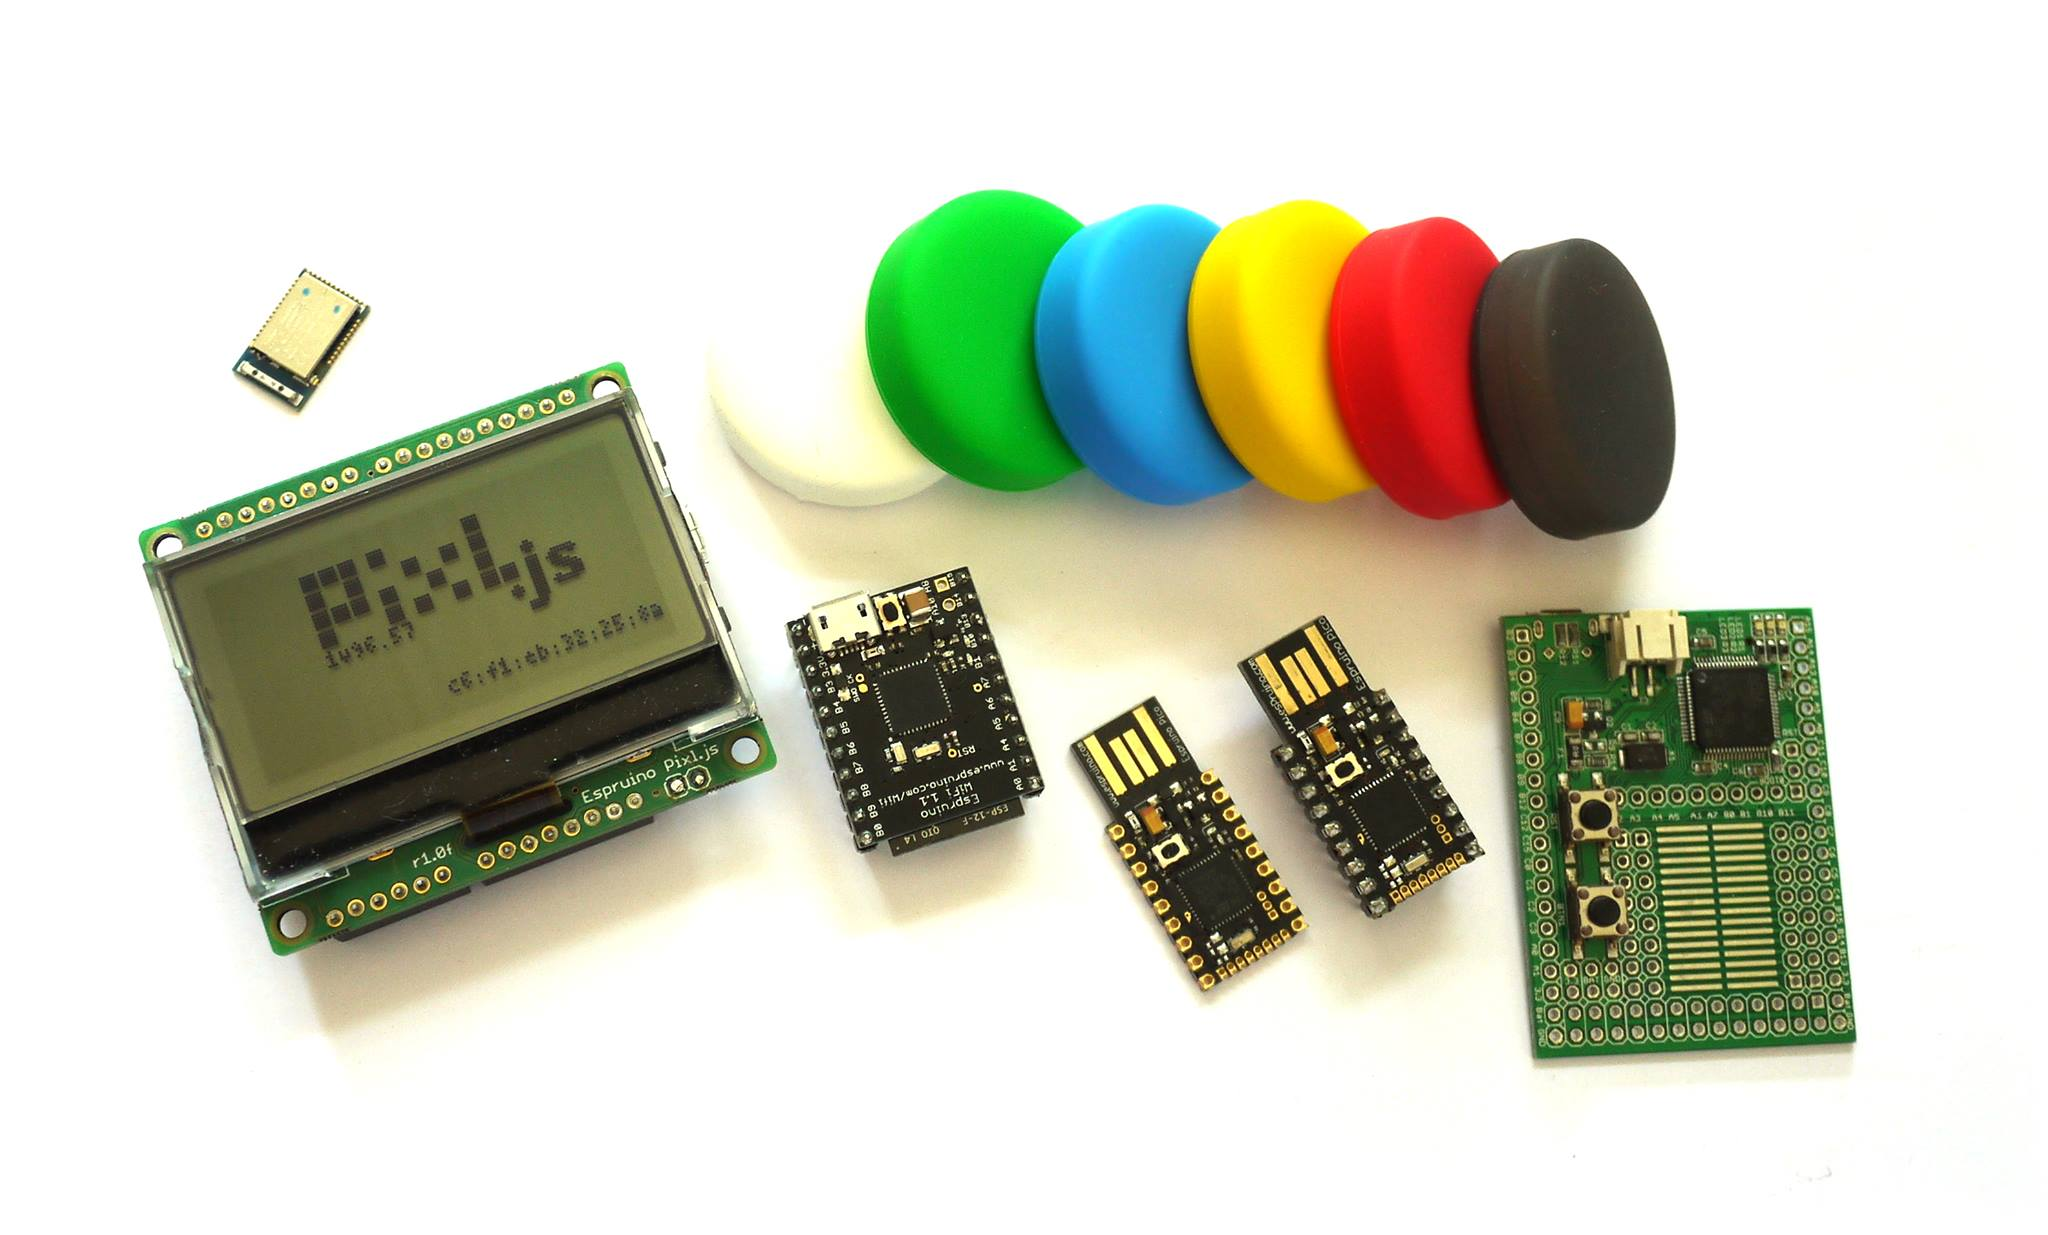
\includegraphics[width=10cm]{dissertation/images/espruino_devices.jpg}
    \caption{Espruino devices}
    \label{fig:espruinodevices}
\end{figure}
    
\subsection{UART}
\text Espruino devices communicate with the browser by utilizing the \href{https://erg.abdn.ac.uk/users/gorry/eg3576/UART.html}{UART protocol}, or Universal Asynchronous Receiver/Transmitter, a widely used communication protocol in the world of micro-controllers and embedded systems. It doesn't require a fixed clock rate between the sender and receiver and instead uses start and stop bits for data transmission synchronization. UART works by utilizing a transmission control line (TX) and a reception control line (RX); UART will begin by sending a start bit from TX to RX to initiate the start of a data transfer from here, data is transferred bit by bit over a single data line starting with the least significant bit (LSB) and finishing with the most significant bit (MSB) following this a stop bit is sent to signal data transfer has finished. This is detailed in figure \ref{fig:UART}.

\begin{figure}[!ht]
\begin{center}
    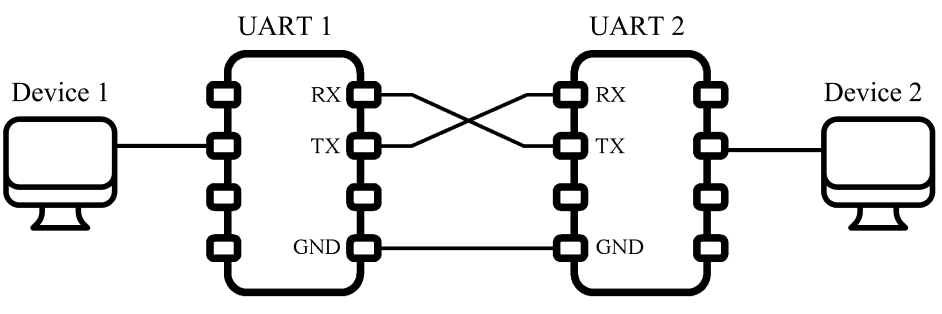
\includegraphics[width=10cm]{dissertation/images/UART_diagram.png}
\end{center}
\caption{UART}
    \label{fig:UART}
\end{figure}

\subsection{WebBluetooth}
\text UART connection with a web browser is facilitated via \href{https://developer.mozilla.org/en-US/docs/Web/API/Web_Bluetooth_API}{WebBluetooth}. WebBluetooth is an aspect of the Web API that facilitates communication between web applications and Bluetooth Low Energy (BLE) devices. This technology allows web developers to control and access BLE devices using JavaScript, providing a streamlined and standardized approach.

WebBluetooth represents a milestone in integrating BLE devices into the web. It offers a common platform for web developers to interact with these devices, regardless of origin or operating system. It expands the possibilities for BLE devices, including the ability to control smart home technology or track fitness information through a web application.

\section{Package Development}

Software packages are methods of extending the functionality of a given language through externally written code. With the wide adoption of node.js in web development, many package developers have adopted the UNIX philosophy of building clean, modular, transparent, and robust code, \cite{TheArtOfUNIXProgramming}. This is achieved in modern web development through the Node Package Manager(NPM).

\subsection{NPM}
\href{https://www.npmjs.com/}{NPM} \text is a tool utilized in JavaScript programming to manage software packages. It is a centralized hub for individuals to quickly find, install, and handle an extensive collection of libraries and packages for their projects. NPM empowers developers to share their packages and work together on open-source initiatives. Due to its large repository of packages, NPM has become a must-have tool for contemporary JavaScript development.

\subsection{NPX}
\href{https://docs.npmjs.com/cli/v7/commands/npx}{NPX} \text is a tool for executing Node.js packages, including those installed through NPM (Node Package Manager). It allows users to run a package's binary without installing it globally on their system. This is useful for testing packages or trying out new features without affecting other parts of the system. NPX also enables developers to run packages with specific versions rather than relying on the globally installed version. It provides a convenient and efficient way to run packages, making it a popular tool in the Node.js ecosystem.

\section{Device to device communication}

Within web development, the challenge of real-time communication between devices is a tricky subject. Examples of well-implemented real-time communication systems are instant messaging services such as WhatsApp and Facebook Messenger or \href{https://developer.mozilla.org/en-US/docs/Glossary/VoIP}{Voice over Internet Protocol (VoIP)} services such as Zoom. These services all have a theme of utilising either \href{https://developer.mozilla.org/en-US/docs/Web/API/WebSocket}{Web-Sockets} or \href{https://developer.mozilla.org/en-US/docs/Glossary/P2P}{Peer to Peer (P2P)} connection.

\subsection{WebRTC}
\href{https://developer.mozilla.org/en-US/docs/Web/API/WebRTC_API}{WebRTC (Web Real-Time Communication)} \text is a freely available resource that enables web browsers and devices to communicate voice, video, and data in real-time without the need for additional software. This technology has been engineered to operate on various networks and platforms, resulting in low lag and excellent audio and video streaming quality for web-based communication. Popular uses for WebRTC include video conferencing, live streaming, online gaming, and file sharing. WebRTC stands out from the crowd by allowing users to connect through a standardized Peer to Peer connection; this skips the requirement of sending messages from a user to a server and then back to a different user and instead uses an external server for signalling a service that helps locate and connect the users. This method reduces server cost due to lowered requests as they are being sent directly from browser to browser.

\begin{figure}[!ht]
    \centering
    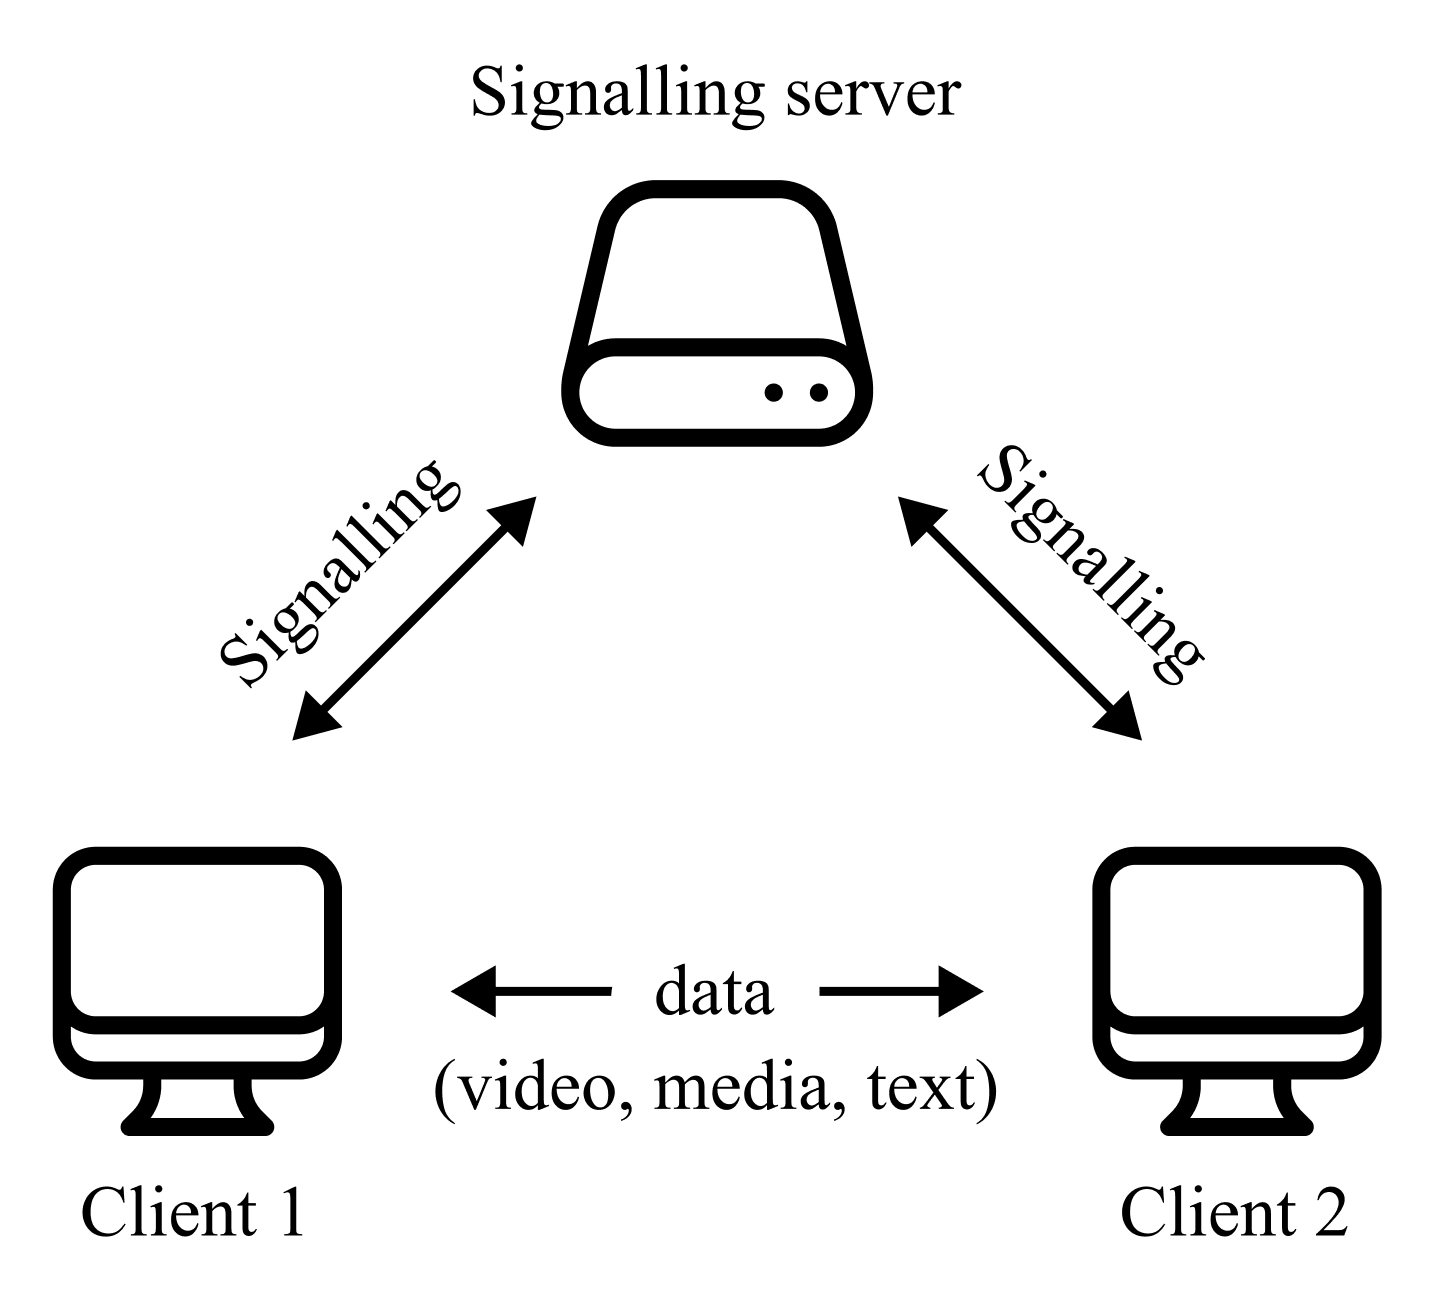
\includegraphics[width=5cm]{dissertation/images/web-rtc-diagram.png}
    \caption{WebRTC}
    \label{fig:webRTC}
\end{figure}

\section{Open Source}
\text Open source pertains to a licensing model for software that enables the public to view and modify the source code. It is developed and maintained by a community of contributors rather than a single entity. Open source aims to promote collaboration, transparency, and innovation in software development and give users more control and choice over their software. Notable open-source projects include the Linux operating system and the Python programming language.

\section{Existing Projects}
\text The Espruino project is an ambitious attempt at bringing embedded systems programming to the masses through an easy-to-get-started ecosystem which takes advantage of many in-house tools to provide the best experience possible for the developers. These tools aim not to change the way we develop but extend upon it through the usage of the below tools we can see this approach.

\subsection{Espruino JavaScript language}
The \href{https://www.espruino.com/Reference#top}{Espruino native language} is an extension of the standard JavaScript library introducing embedded systems specific keywords such as \textit{SetWatch} and pin manipulation through the syntax \textit{PIN.method()}. Adding these keywords allows developers to interact and control embedded devices in a manner akin to alternatives such as Arduino or Micro Python. This extension of the language transforms JavaScript into a capable systems programming language aimed at Espruino microcontroller boards.

\subsection{Espruino IDE}
The \href{https://www.espruino.com/ide/}{Espruino IDE} provides an online platform for developers to get started working with their Espruino devices without the need to set up any local environments. This web application provides many features, such as device console logs and programming directly onto the device all around providing a perfect learning environment for new programmers and acting as an ideal debugging environment for more experienced developers.

\begin{figure}[!ht]
    \centering
    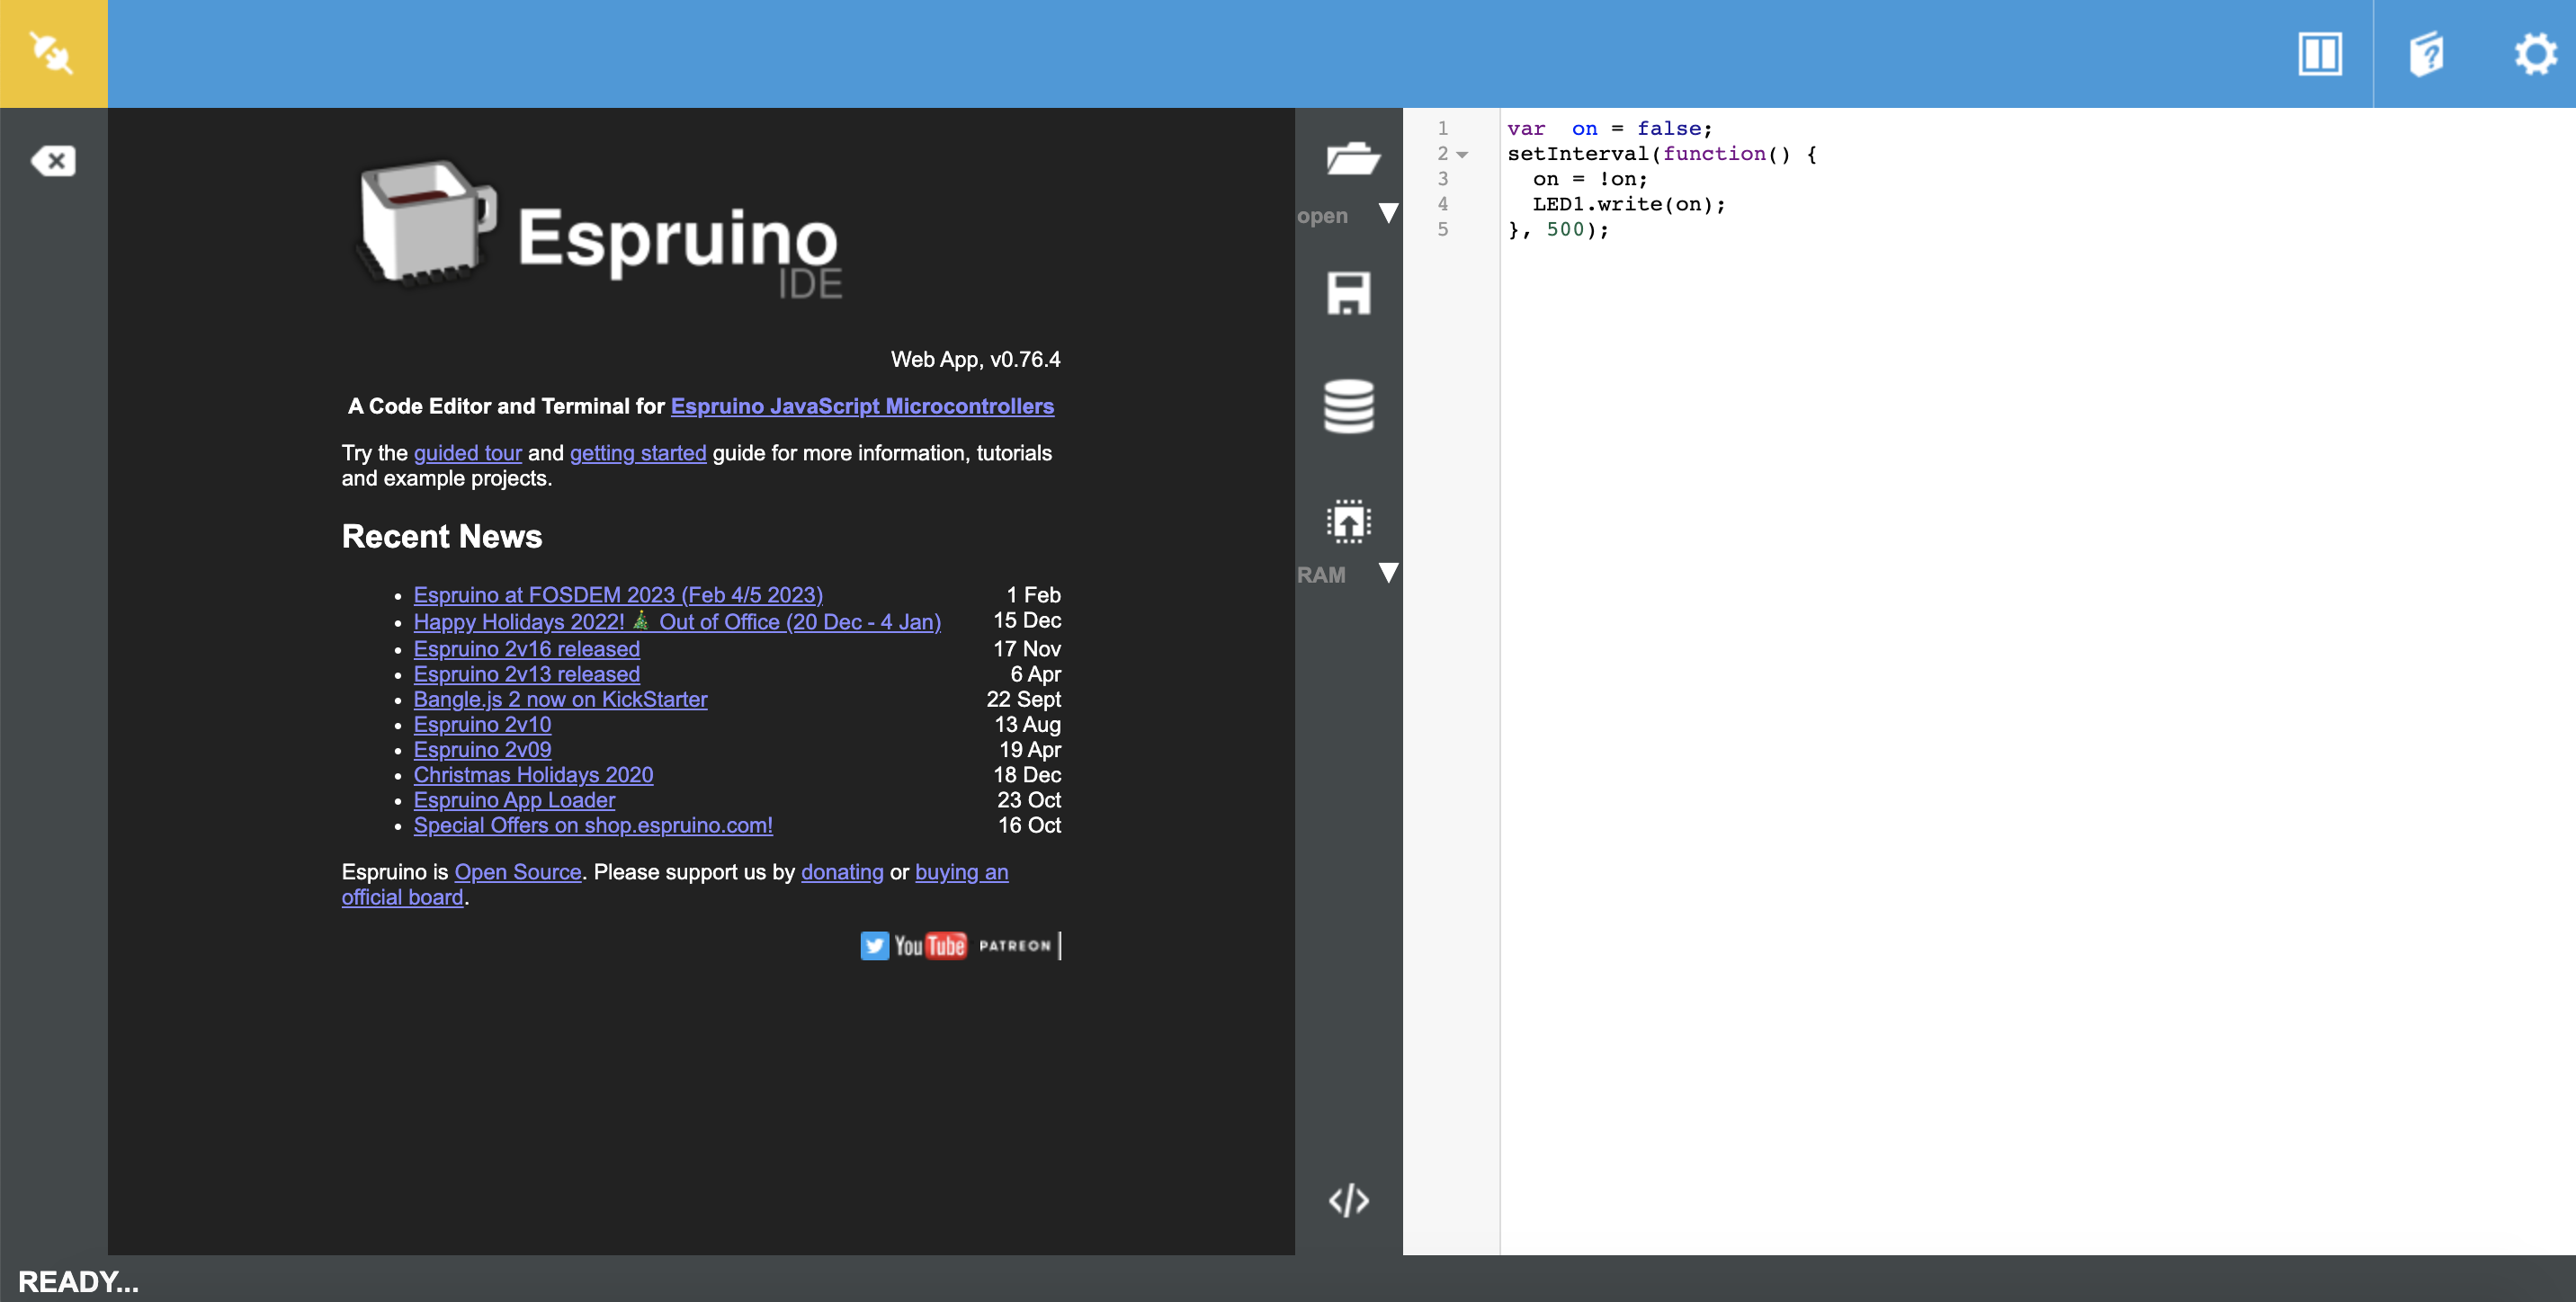
\includegraphics[width=10cm]{dissertation/images/espruino-ide.png}
    \caption{Espruino IDE}
    \label{fig:espruino-ide}
\end{figure}

%==================================================================================================================================
\chapter{Analysis/Requirements}

\text Due to the nature of this project having multiple smaller packages/applications, these mini projects were analysed separately. To accomplish this, a MOSCOW analysis was undertaken on each project individually. Below is a compilation of the main points from this individual analysis, including overlapping themes and essential points from each project with the complete MOSCOW requirements for each project referenced within the appendix \ref{appendix:MOSCOWAnalysis}.

\section{Problem specification}
The Espruino platform provides an unopinionated approach to how users should use their platform, resulting in less-than-perfect tools being used out of necessity. These tools are uninviting for new programmers and lack many features for experienced programmers, a few examples of which are shown below.

\begin{itemize}
    \item easily control embedded device from the web page with the ability to gather device data.
    \item adds the ability to use an Espruino device as a JavaScript module.
    \item develops an environment which allows both beginners and experienced programmers to work with remote embedded devices, i.e. no limitations with straightforward syntax.
    \item removes the need to write code as a string to send to the device. With the current implementation, an approach as shown in figure \ref{fig:OLD_UART_DEVICE_WRITING_CODE} has to be taken. This removes both auto-complete functionalities and makes code less readable.

    \begin{figure}[!ht]
        \begin{lstlisting}
            import UART from 'uart.js';
        
            let code = `setWatch(function () {
                    LED1.set();
                }, BTN, {
                    edge: 'rising',
                    repeat: true,
                    debounce: 50
                })`;

            UART.write(`${code};\n`);
            
        \end{lstlisting}
        \caption{UART.js device communication}
        \label{fig:OLD_UART_DEVICE_WRITING_CODE}
    \end{figure}

     An additional issue with this approach is the requirement to end all code with a new line, as the interpreter will not execute the code otherwise. The code should be written as standard with code completion within the IDE. An example of how this could be done is shown in figure \ref{fig:NEW_DEVICE_WRITING_CODE}. An approach allows fewer errors at run time due to syntax highlighting. 

     \begin{figure}[!ht]
        \begin{lstlisting}
            import Device from 'new_package';

            let device = new Device()
        
            device.setWatch(function () {
                    device.LED1.set();
                }, device.BTN, {
                    edge: 'rising',
                    repeat: true,
                    debounce: 50
                })`;
            
        \end{lstlisting}
        \caption{Proposed new device communication}
        \label{fig:NEW_DEVICE_WRITING_CODE}
    \end{figure}
\end{itemize}

\section{Functional Requirements}
The problem specification provided a platform allowing for an open-ended approach to the problem at hand. By taking an approach that aimed to improve the current approaches taken whilst creating a platform that encouraged beginner programmers to get involved and learn. The following breakdown is the result of these considerations.
% Short paragraph explaining the breakdown of the work items from the original specification
\subsection{Must Have}
\begin{itemize}
    \item A fully open-source ecosystem to allow for community contribution and overall clarity of how the project works at the code level.
    \item Clean and accessible syntax for the end developer to get started with, including inline documentation through IDE comments.
    \item Improve the development process of the Espruino device by introducing a modular programming method compared to the current almost terminal-based approach.
\end{itemize}
\subsection{Should Have}
\begin{itemize}
    \item Support any style favoured programming style, including but not limited to JavaScript frameworks. A practice that will not discourage programmers at any level from jumping into something they are already familiar or comfortable with. This will include imports through script flags as well as NPM.
    \item Refined user interface to ensure integration into existing sites is not a hassle nor an eyesore. This should be consistent across all products.
\end{itemize}
\subsection{Could Have}
\begin{itemize}
    \item Easily extendable packages, including only the core functionality of the packages, to allow developers to extend and implement desired features without being held back by any limitations.
\end{itemize}
\section{Non-Functional Requirements}
\text The project aims to improve the Espruino platform whilst providing beginners a platform to grow their programming skills. An important aim is to produce an ecosystem of clear instructions and examples to follow along and fully understand what the platform is capable of.
\subsection{Must Have}
\begin{itemize}
    \item A well-populated documentation site to explain the ins and outs of each package in depth.
    \item A hub for users to explore in-depth projects built on the espruino-tools platform whilst allowing them to show off their creations to the public.
    
\end{itemize} 
\subsection{Should Have}
\begin{itemize}
    \item Easy contribution from the open-source community through the usage of modern standards and clear, clean code.
    \item A platform with online guides and videos which clearly walk the developer through the process of building a project allowing beginners to get started with functioning examples whilst letting them explore the intricacies of the package.
\end{itemize} 

\section{Specification changes}

\text As this project was very open-ended and heavily incorporated user testing, it allowed for an approach where feedback generated what was happening next. Through the development process, many smaller projects were built to improve the development experience; below are the significant changes to the original specification; each breakdown in the specification is expanded further through complete MOSCOW analysis within appendix \ref{appendix:MOSCOWAnalysis}.

\subsection{Peer to Peer}
\text During the development of the main package, a discussion occurred surrounding the limitations of the WebBluetooth API. As WebBluetooth is a new technology, the support for it is restricted; by viewing the \href{https://caniuse.com/?search=WebBluetooth}{caniuse} tool shown in figure \ref{fig:caniuse_webblue} we can see that only chromium based browsers support this API with no direct support for iOS devices.

\begin{figure}[!ht]
    \centering
    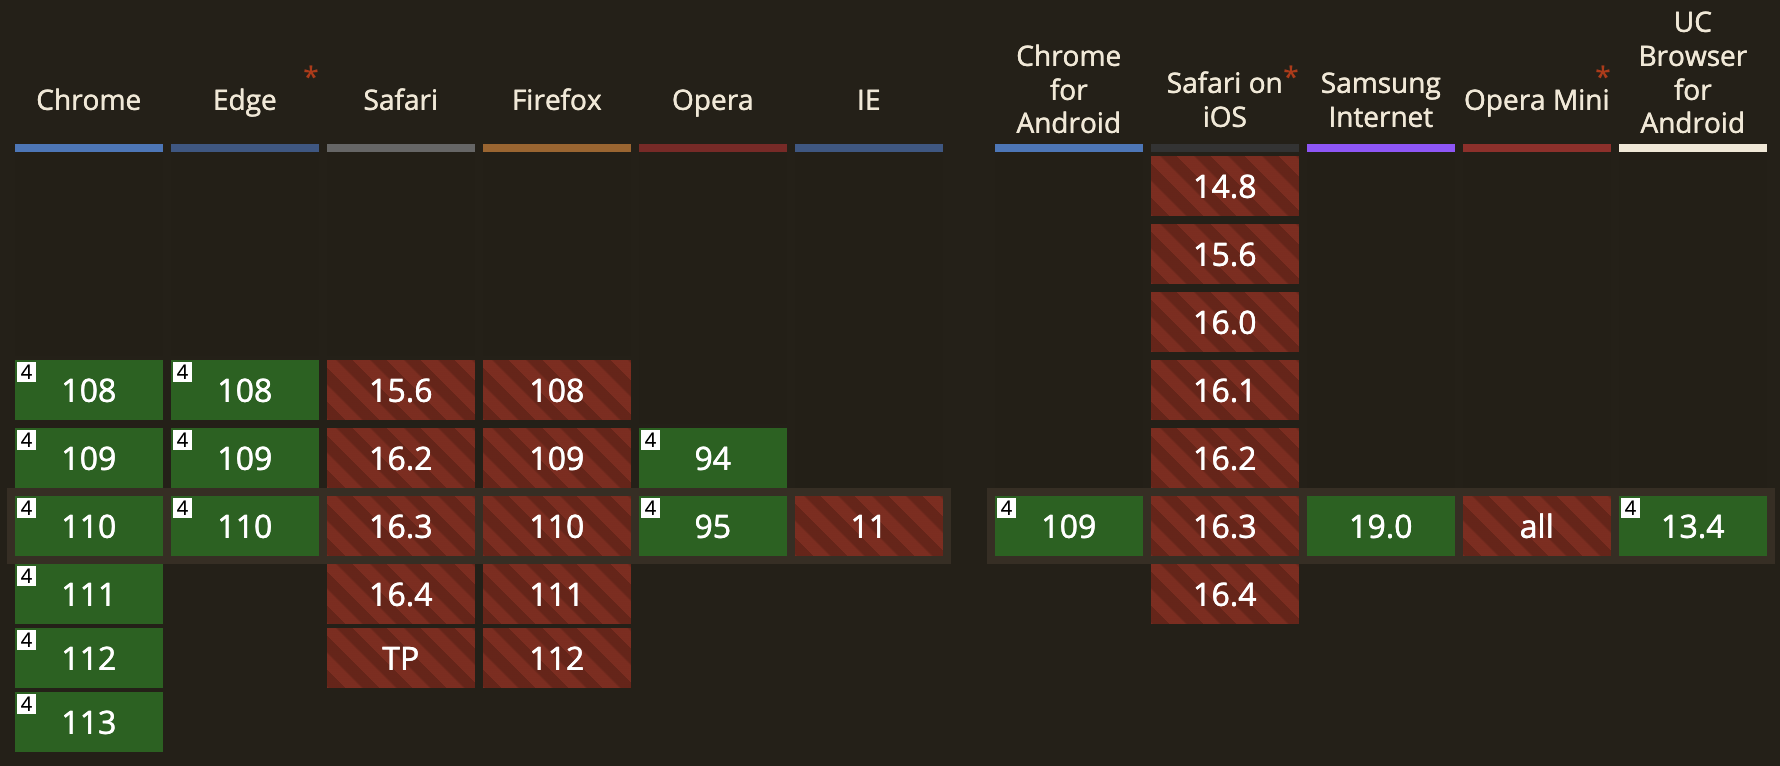
\includegraphics[width=12cm]{dissertation/images/caniuse_webbluetooth.png}
    \caption{caniuse WebBluetooth adoption}
    \label{fig:caniuse_webblue}
\end{figure}

A problem this presents is that \href{https://gs.statcounter.com/os-market-share/mobile/united-kingdom}{statcounter}'s Mobile Operating System Market Share United Kingdom states that more than half (52.44\%) of smart device users are on iOS devices as shown in figure \ref{fig:smartdeviceusage}\\\\

\begin{figure}[!ht]
    \centering
    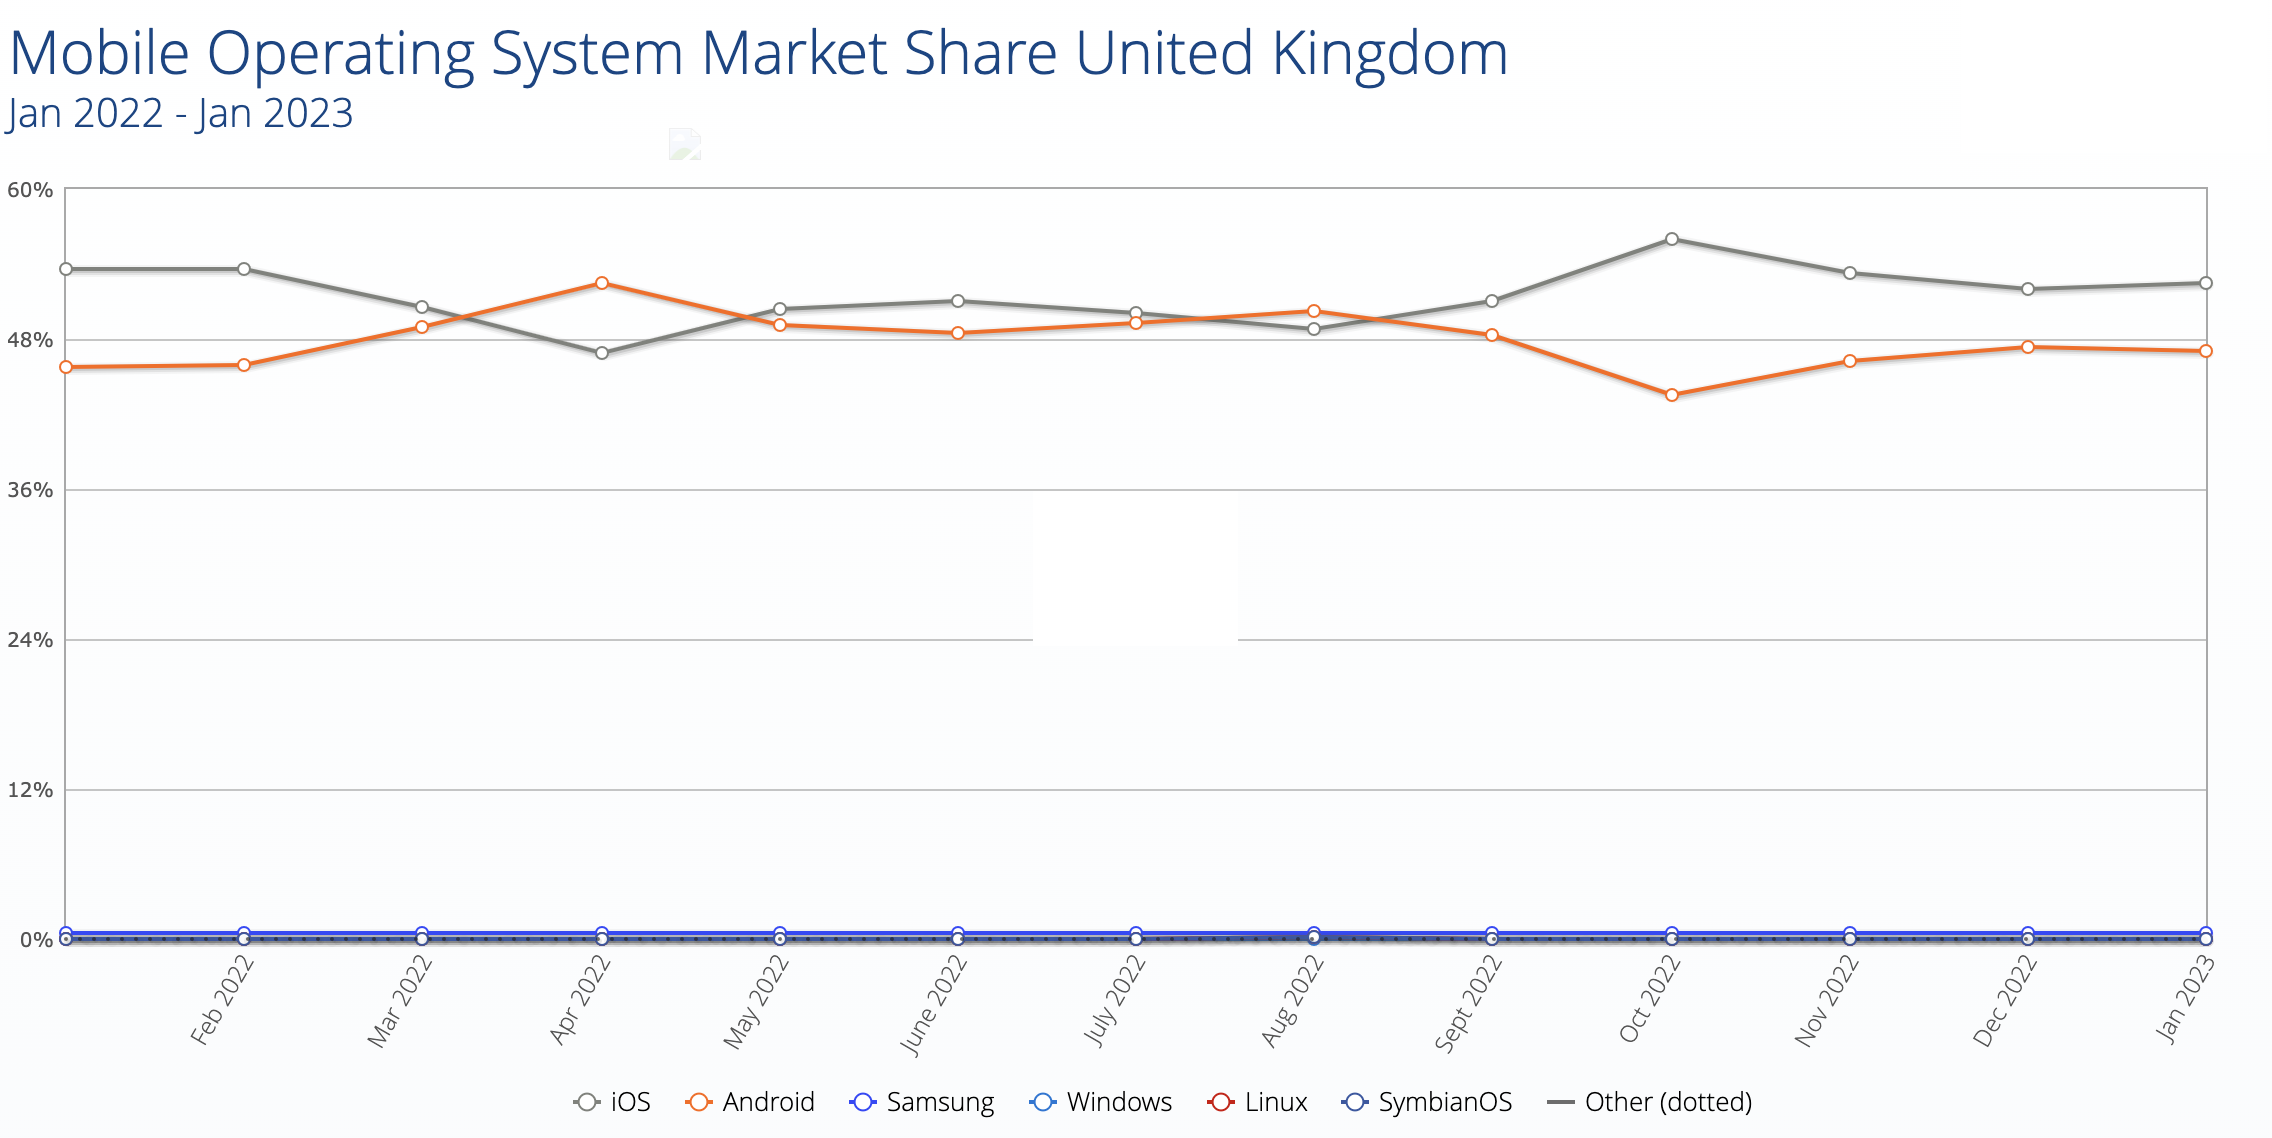
\includegraphics[width=12cm]{dissertation/images/mobile-operating-system-usage.png}
    \caption{Mobile Operating System Market Share United Kingdom (Jan 2022 - Jan 2023)}
    \label{fig:smartdeviceusage}
\end{figure}

Smartphones may be used within the remote embedded systems space due to the limitations of the device. Mobile phones present multiple input and output interfaces that Espruino devices do not have such as cameras (used in tracking), microphones (used in voice commands), or even touch controls that allow for a more comprehensive feature set than the simple buttons provided.
\\ 

To bypass this issue and allow unsupported control over these devices, a solution of utilising a peer-to-peer communication package made sense allowing unsupported devices to connect to a main supported device as shown in figure \ref{fig:mobile-computer-connection}. 

\begin{figure}[!ht]
    \centering
    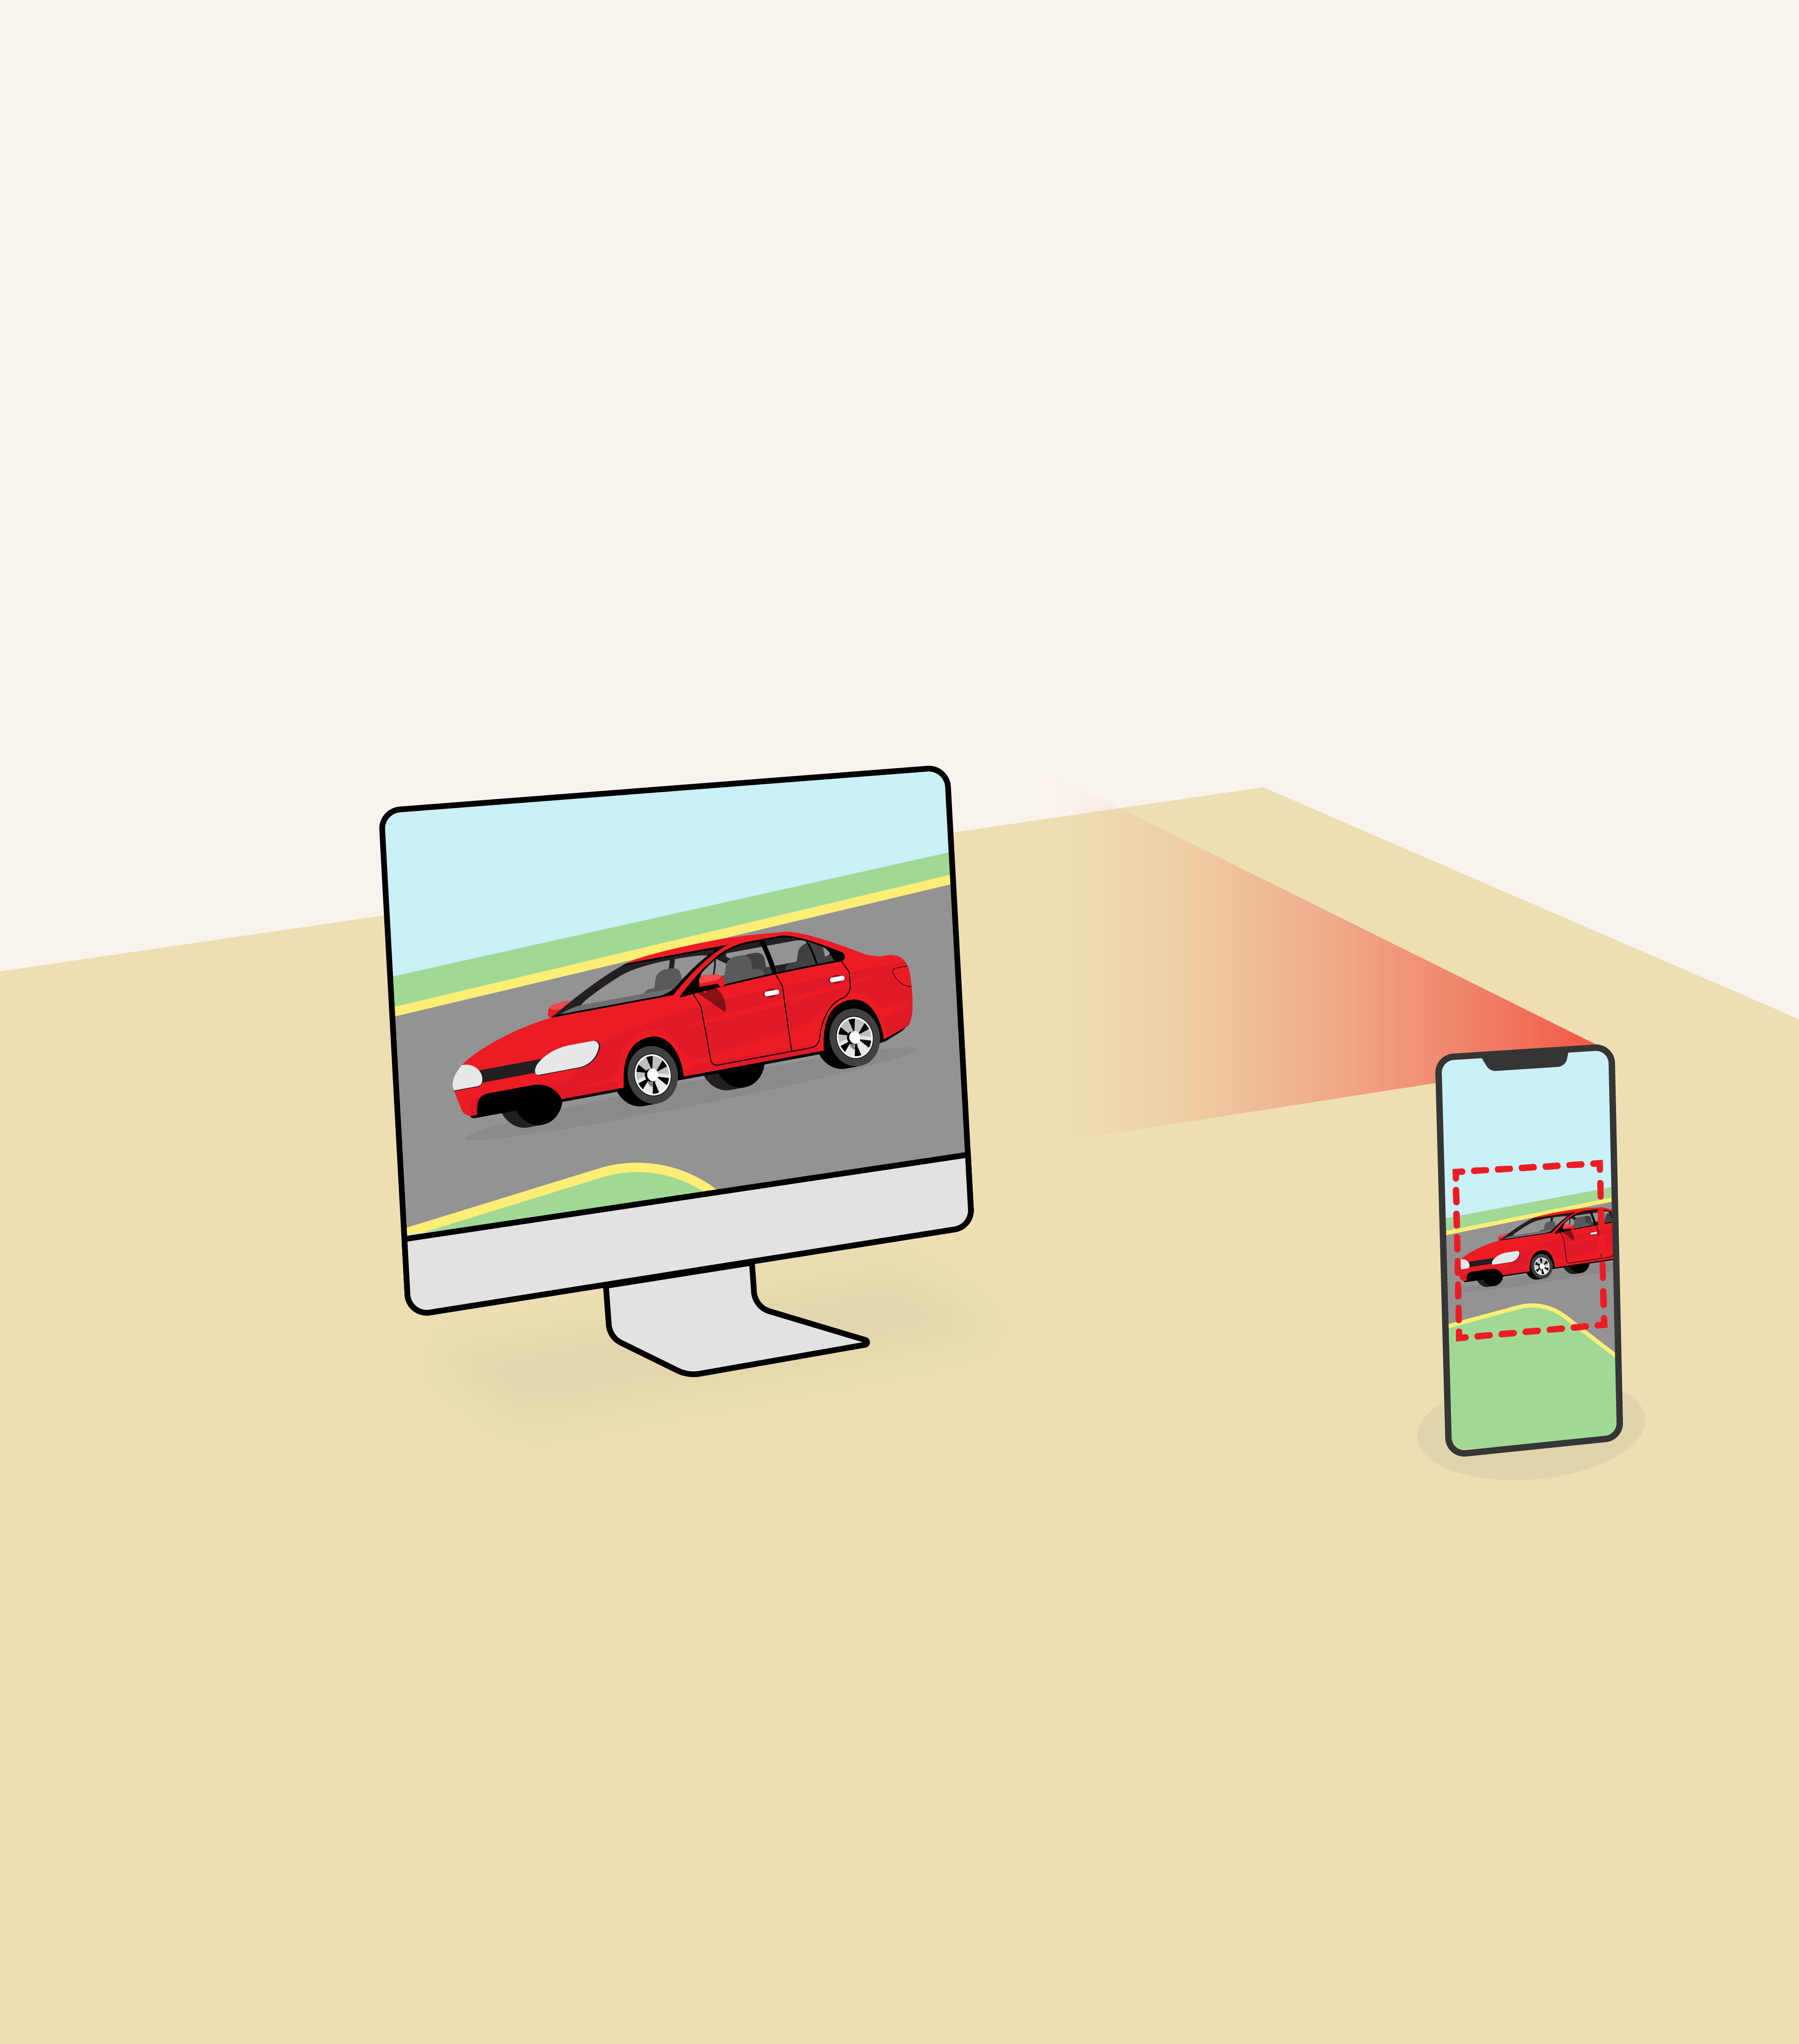
\includegraphics[width=7cm]{dissertation/images/mobile-computer-connection.png}
    \caption{Mobile - Computer connection}
    \label{fig:mobile-computer-connection}
\end{figure}

This approach was taken to allow users with iOS devices to control espruino devices, expanding the scope of projects available to a broader audience. To incorporate this, it would need to have the following specifications:
\\
\begin{itemize}
    \item Support for any mobile device type, including but not limited to iOS and Android devices.
    \item Simplify the integration of peer-to-peer focusing on sending data and video whilst not restricting developer freedom.
    \item Utilise an automatically generated QR code to allow easy device connection through the camera of a mobile device.
\end{itemize}

\subsection{Transpiler}
As the main project began to incorporate more complex behaviour like nested statements for anonymous functions which contain scope code within them. This presented an issue where the previous approach of a mini parser utilised a map of possible espruino methods along with string manipulation to replace known configurations that could come up. This approach had a few problems, such as no freedom to name instances of espruino devices as well as no support for the use of variables or nested scoped code. This approach to solving the problem ended up making the development experience worse, going directly against the aims of the project. The following code was not possible in the original approach.

\begin{lstlisting}
    import { Puck } from '@espruino-tools/core';

    let my_custom_puck_name = new Puck();
    
    my_custom_puck_name.onPress(async () => {
    
        let light_val = await my_custom_puck_name.getLightVal()
        
        if(light_val){
            my_custom_puck_name.LED.on("red");
        } else {
            my_custom_puck_name.LED.off("red");
        }
    })
\end{lstlisting}

To solve this problem, an approach which took inspiration from transpiled languages such as TypeScript made the most sense. A Transpiler, in this case, allowed a new language to be built extending JavaScript's syntax this could then be compiled into plain JavaScript, which could be interpreted by Espruino's compiler. For the transpiler to be effective, it had to ensure to incorporate the following criteria.
\\
\begin{itemize}
    \item successfully converts all standard JavaScript allowing for variable declaration, nested scoped code as well as imports/exports.
    \item Allow for code written in either standard Espruino language or the new Espruino tools syntax for niche unsupported methods to not be restricted.
    \item Support modern JavaScript programming including modules, classes and syntax such as arrow functions or async/await.
\end{itemize}

\subsection{NPX Tool}
\text By expanding the espruino platform to the NPM platform it became apparent that the setup of the package directory may become cumbersome for more experienced developers or downright difficult for beginner programmers with no previous node.js knowledge. By taking inspiration from React's \href{https://reactjs.org/docs/create-a-new-react-app.html}{create-react-app} tool it made the most sense to approach the problem in the same way by allowing users a simple command line prompt with avid customisation to allow a default project which fits the needs of most developers leaving heavily customised projects to the audience of people that needed it. To incorporate this, it would need to have the following specifications:
\\
\begin{itemize}
    \item Create a working directory to allow users to get started directly after the command is run with no additional setup.
    \item An effective build command to convert users' node.js project into its respected static files for easy hosting and sharing of projects.
    \item Support for different JavaScript development approaches, including frameworks such as React and Vue or just plain JavaScript solutions such as vanilla JavaScript or TypeScript.
\end{itemize}

\subsection{Online Environment}
\text The original Espruino project includes an online environment which allows users to develop straight onto their Espruino devices removing the need to set up a local environment to test smaller features. As this project utilises a new syntax whilst bringing many useful development tools such as gathering device code effectively, it made sense to take inspiration from the Espruino IDE and create an environment which supports this new style of programming on Espruino devices whilst incorporating functionality aimed at improving the experience for developers. For this aspect of the project to be effective it had to meet the following criteria:
\\
\begin{itemize}
    \item It must support live development with the ability to run code and see device output to allow developers to catch any bugs that may be missed in standard development.
    \item Bring the ability for users to upload and download their code to allow easy integration into a larger project be that through debugging or just testing features first before bringing them into the project.
    \item Allow users to directly see device code in a read-only code editor, allowing an improved debugging experience for developers.
\end{itemize}

% Allow users to have an environment in which they can test new features without setting up a whole development environment. This can be used to test functionality or even develop whole projects.
%==================================================================================================================================
\chapter{Design}

\section{Development}

Throughout the development of this project, multiple development approaches have been taken based on the project style. By utilising both a feedback-driven model alongside a test-driven approach, each aspect of the project has been allocated an appropriate development style to ensure robustness, cleanness and adequate feature sets. These approaches were enforced using agile methodologies by dividing specification points into work items and allocating them during week-long sprints furthering the quick approach to iterating the product.

\subsection{Feedback Driven Development}
By utilising a feedback-driven approach the project was able to constantly evolve into a product more suited to the people actually using it. To take full advantage of the Espruino community and ensure the project provided useful features three methods of gathering feedback were used.

\text \\

\subsubsection{Espruino Forum}\hfill\\
The Espruino Forum pictured in figure \ref{fig:espruino-forum} is a platform used by the community to share new projects or to ask for help with problems ran into within the development cycle. The forum allowed for direct communication with Gordan Williams the creator of the Espruino platform. Discussion and feedback on the shared project allowed for further iterations of the project to be made.

\begin{figure}[!ht]
    \centering
    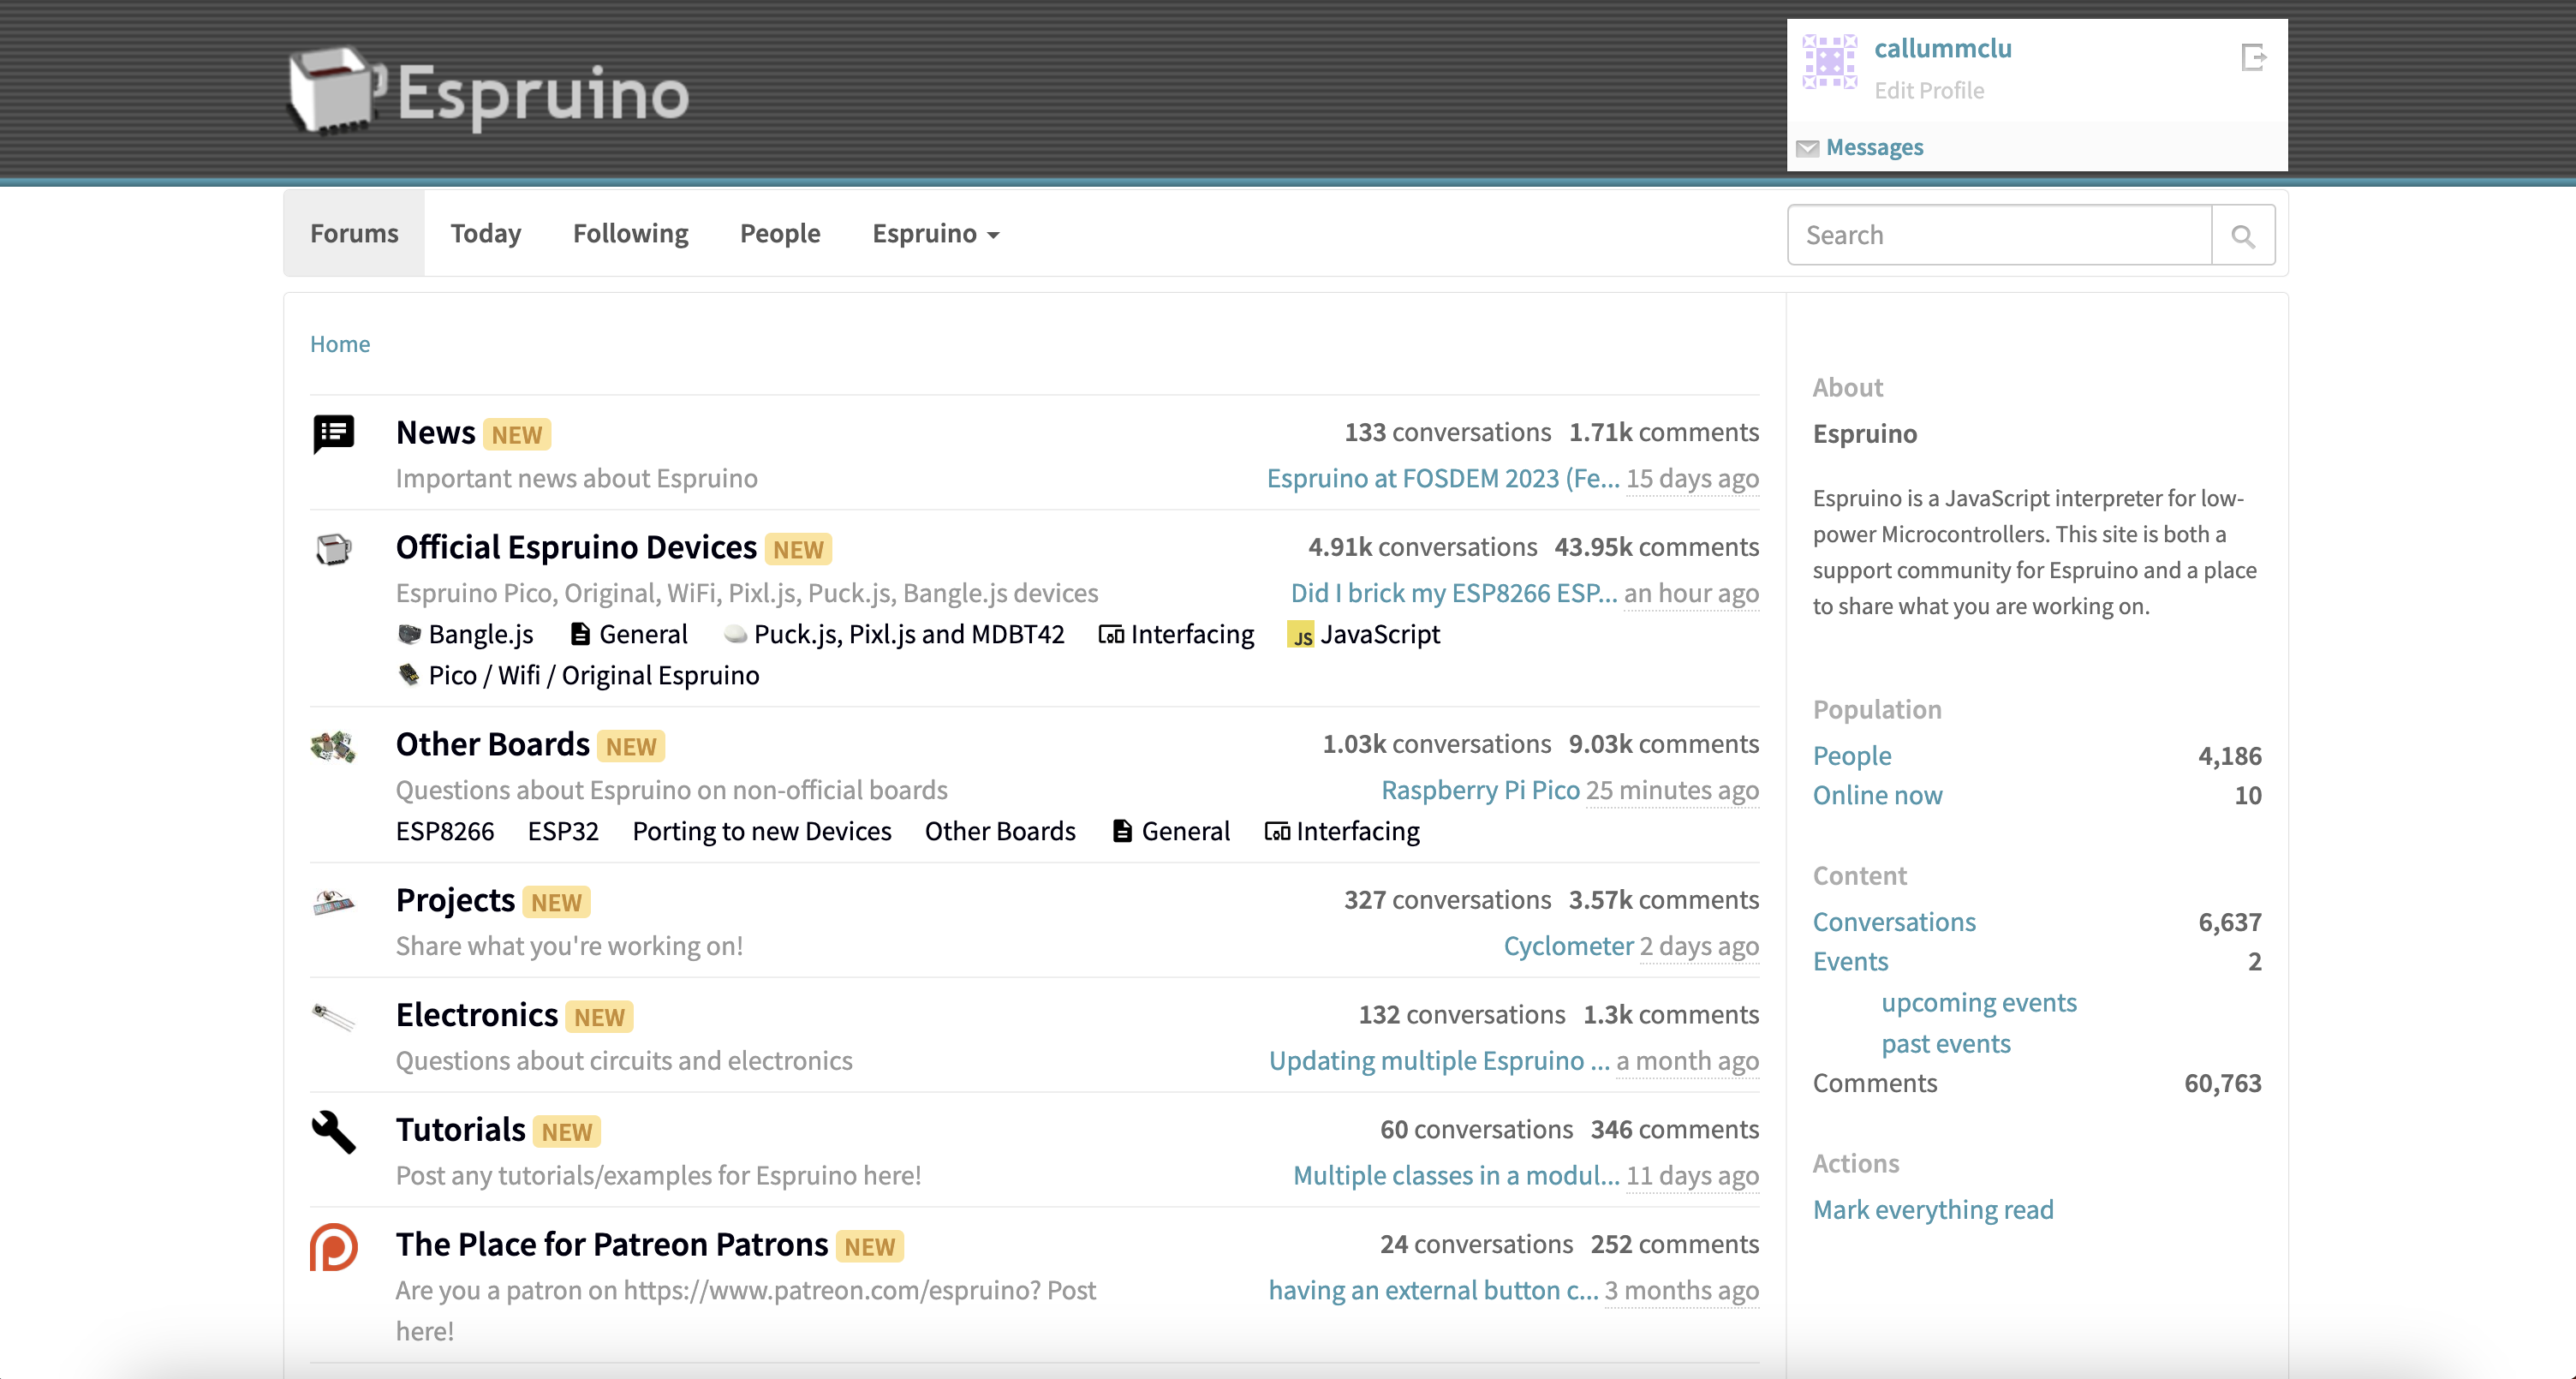
\includegraphics[width=12cm]{dissertation/images/espruino-forum.png}
    \caption{Espruino Forum}
    \label{fig:espruino-forum}
\end{figure}

\text \\
\subsubsection{User testing}\hfill\\
Throughout the full project user testing was utilised allowing a constant flow of feedback from a developer using the packages to build their own substantial project utilising every aspect of the package suite. By incorporating this feedback this vital stage allowed for package-wide user testing as well as both suggestions for feature additions and help with finding bugs within the code.

\text \\
\subsubsection{Supervisor Feedback}\hfill\\
Due to the supervisors' involvement within the Espruino ecosystem through the development of a new espruino device as well as a genuine interest in the products feedback from them was essential. By having somebody who knew about the platform and had an acute interest in the product themselves allowed for many discussion sessions where new features and ideas could be bounced back and forth allowing for a creative environment including new direction ideas or even how features could be improved.

\text \\

This approach allowed for very small iterations to be planned out developed and deployed in a very short period further allowing again for quick feedback surrounding the changes as well as a platform to test prototyped ideas as a smoke test for the final product.


\subsection{Test Driven Development}

Test Driven Development (TDD) is the process of writing failing tests first and ensuring the criteria are met before writing the following tests until the end product is produced. Where possible Test Driven Development was used throughout the full package ecosystem. For all packages, the feedback-driven approach was used in tandem with test-driven development to ensure these feature-rich packages both did not break with massive changes as well as allowing them to maintain substantial test coverage. Overall this approach allowed for the code quality to be constantly improved without worries of breaking previous functionality and played a vital part in the development of the transpiler package and its conversion from the imperfect original core implementation.

\section{Organisations}

By utilising organisations within this project I was able to keep relevant code in a single place; this was important due to the open-source nature of the project by keeping everything together users or contributors are able to navigate the full code base with less hassle.

\subsection{GitHub}
The GitHub platform is widely used within the open-source community, a feature provided by GitHub is GitHub organisations. GitHub organisations provide a workspace that promotes contribution and collaboration through allowed permissions allowing for control over who has access to alter code. 

\text Alongside this Github organisations allows for a project with multiple repositories to be grouped together keeping all relevant code in one place. Doing this allows newer developers to discover both how all the packages work and also see the catalogue of packages offered by the ecosystem. Below in figure \ref{fig:ghorg} we can see the GitHub organisation for this project.

\begin{figure}[!ht]
    \centering
    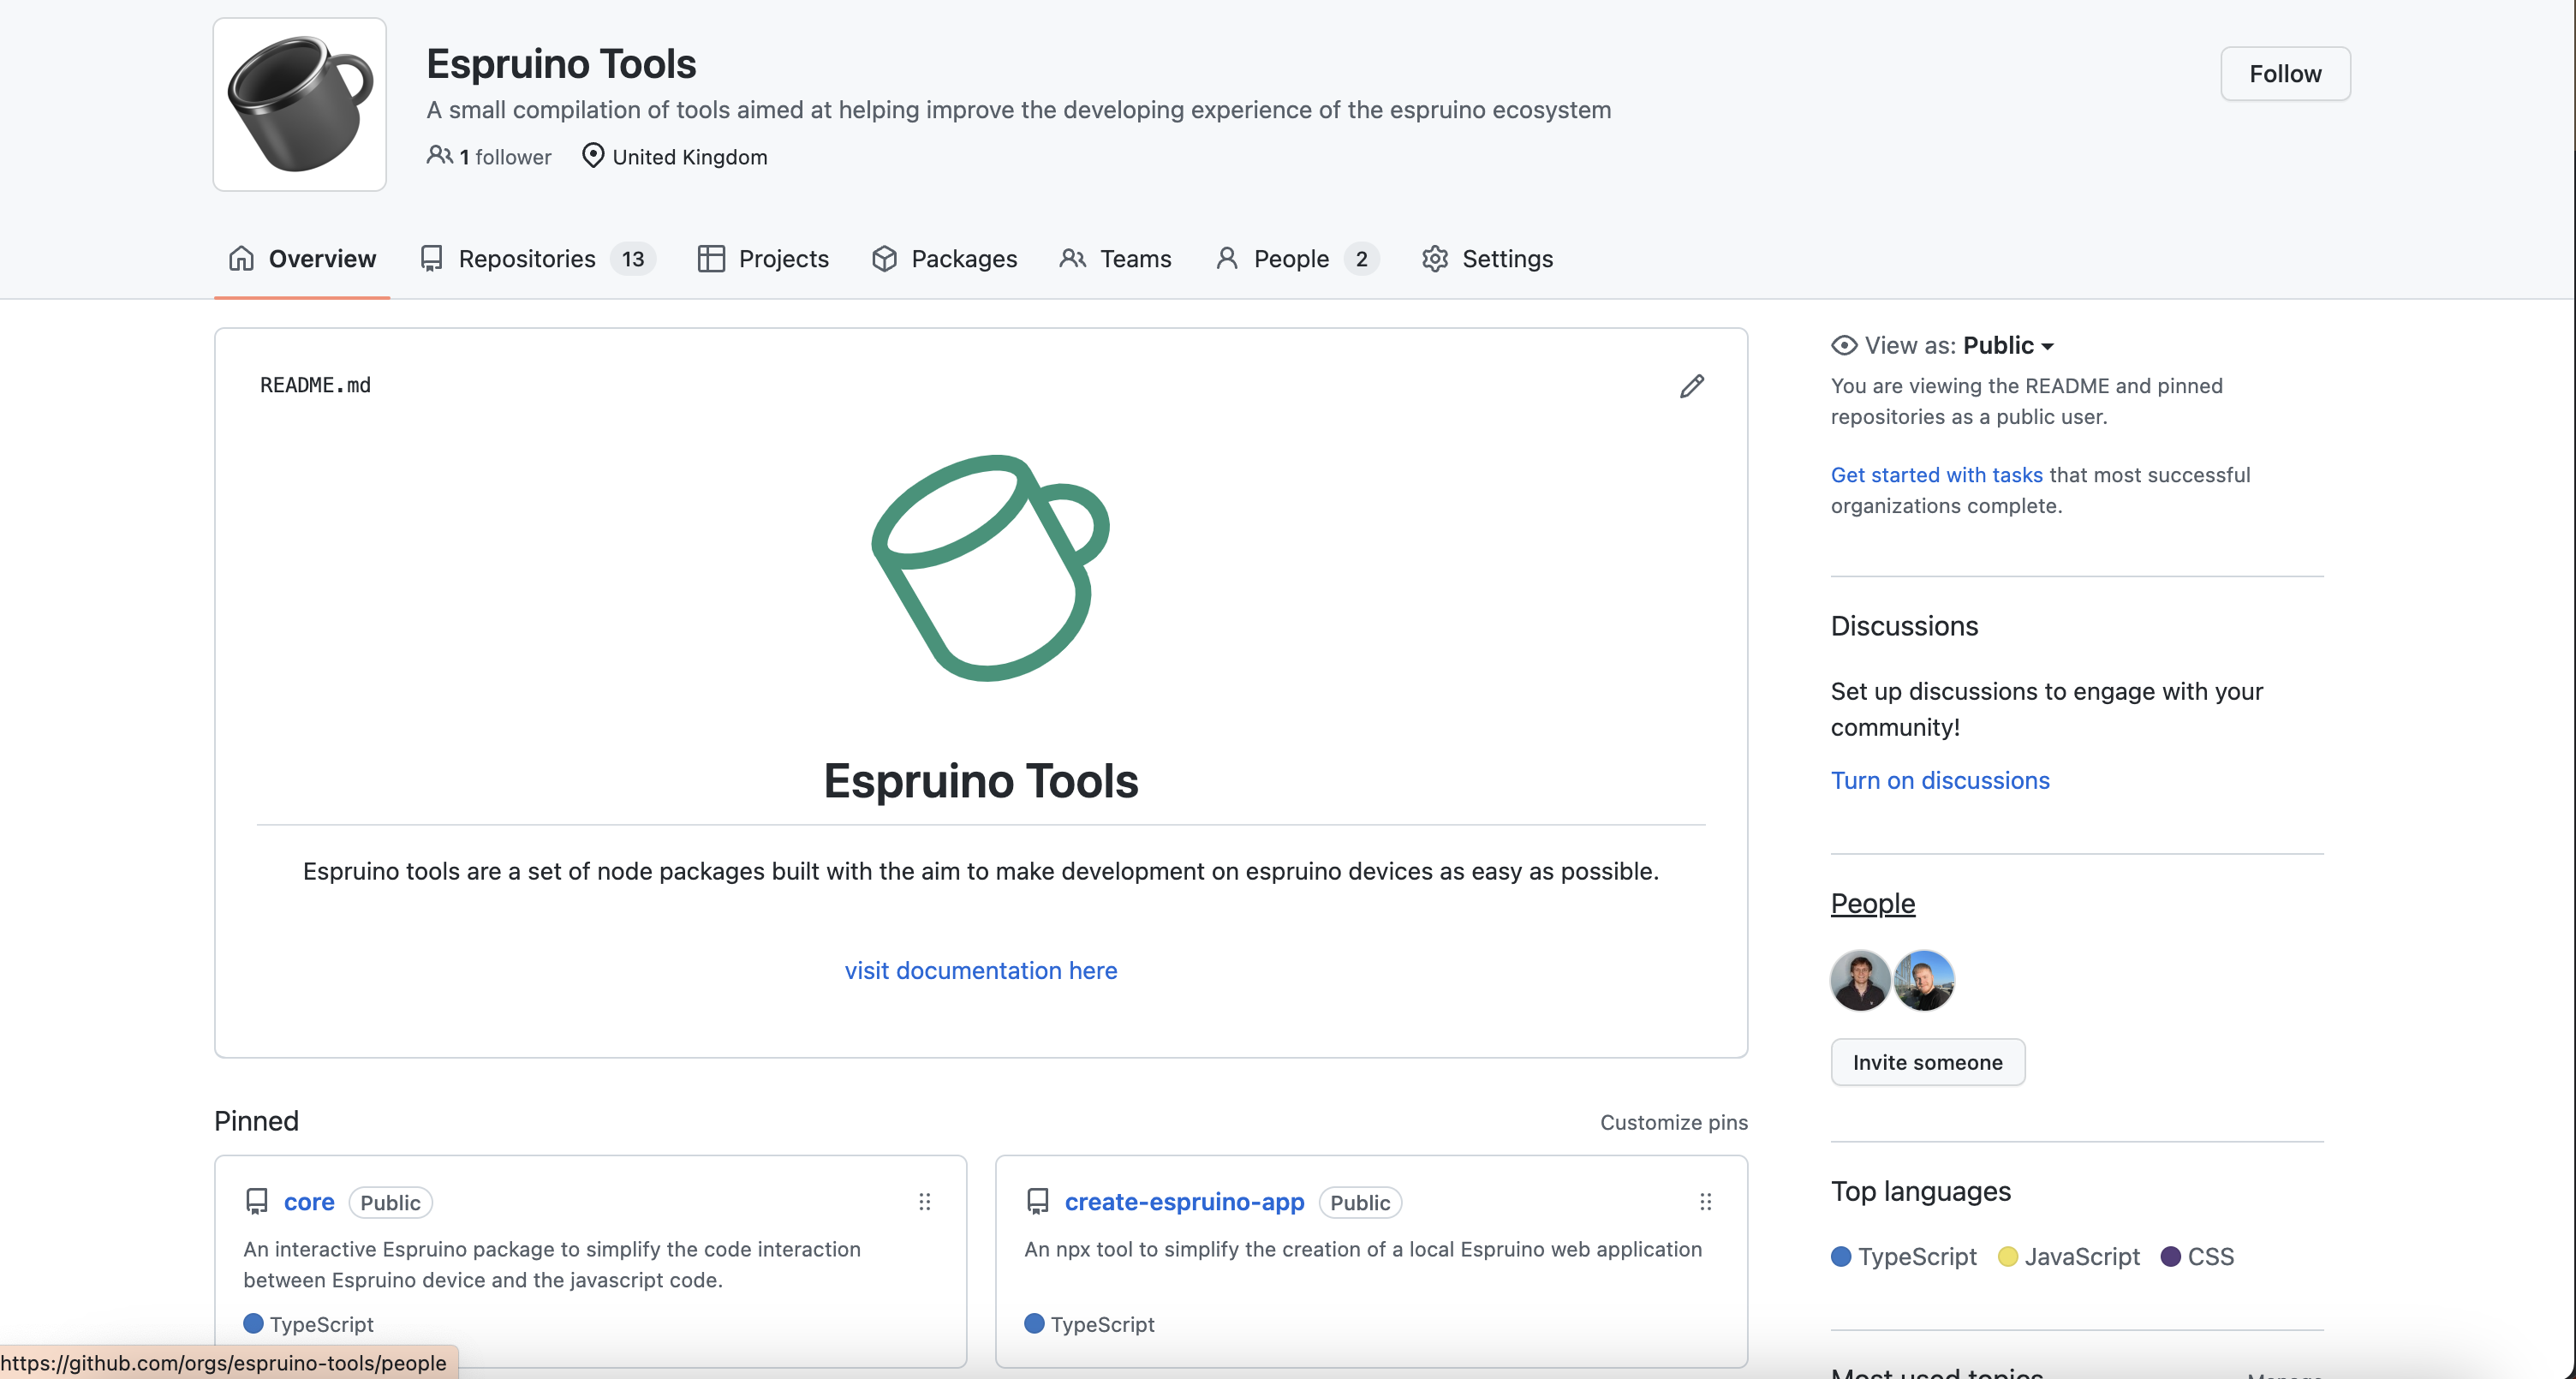
\includegraphics[width=10cm]{dissertation/images/github-organisation.png}
    \caption{\href{https://github.com/espruino-tools}{Github organisation}}
    \label{fig:ghorg}
\end{figure}

\subsection{NPM}

NPM provides a solution similar to GitHub organisations through scoped packages. NPM's scoped packages provide similar benefits such as keeping related code together whilst adding others. One of the main draws to NPM's scoped packages is the ability to name your packages similarly to packages that have previously been built prepending a given organisation's name. This approach avoids cryptic package naming schemes whilst keeping the projects consistent. As seen below in figure \ref{fig:npmorg} each scoped package within the organisation maintains the syntax of \textbf{@espruino-tools/<package-name>}.

\begin{figure}[!ht]
    \centering
    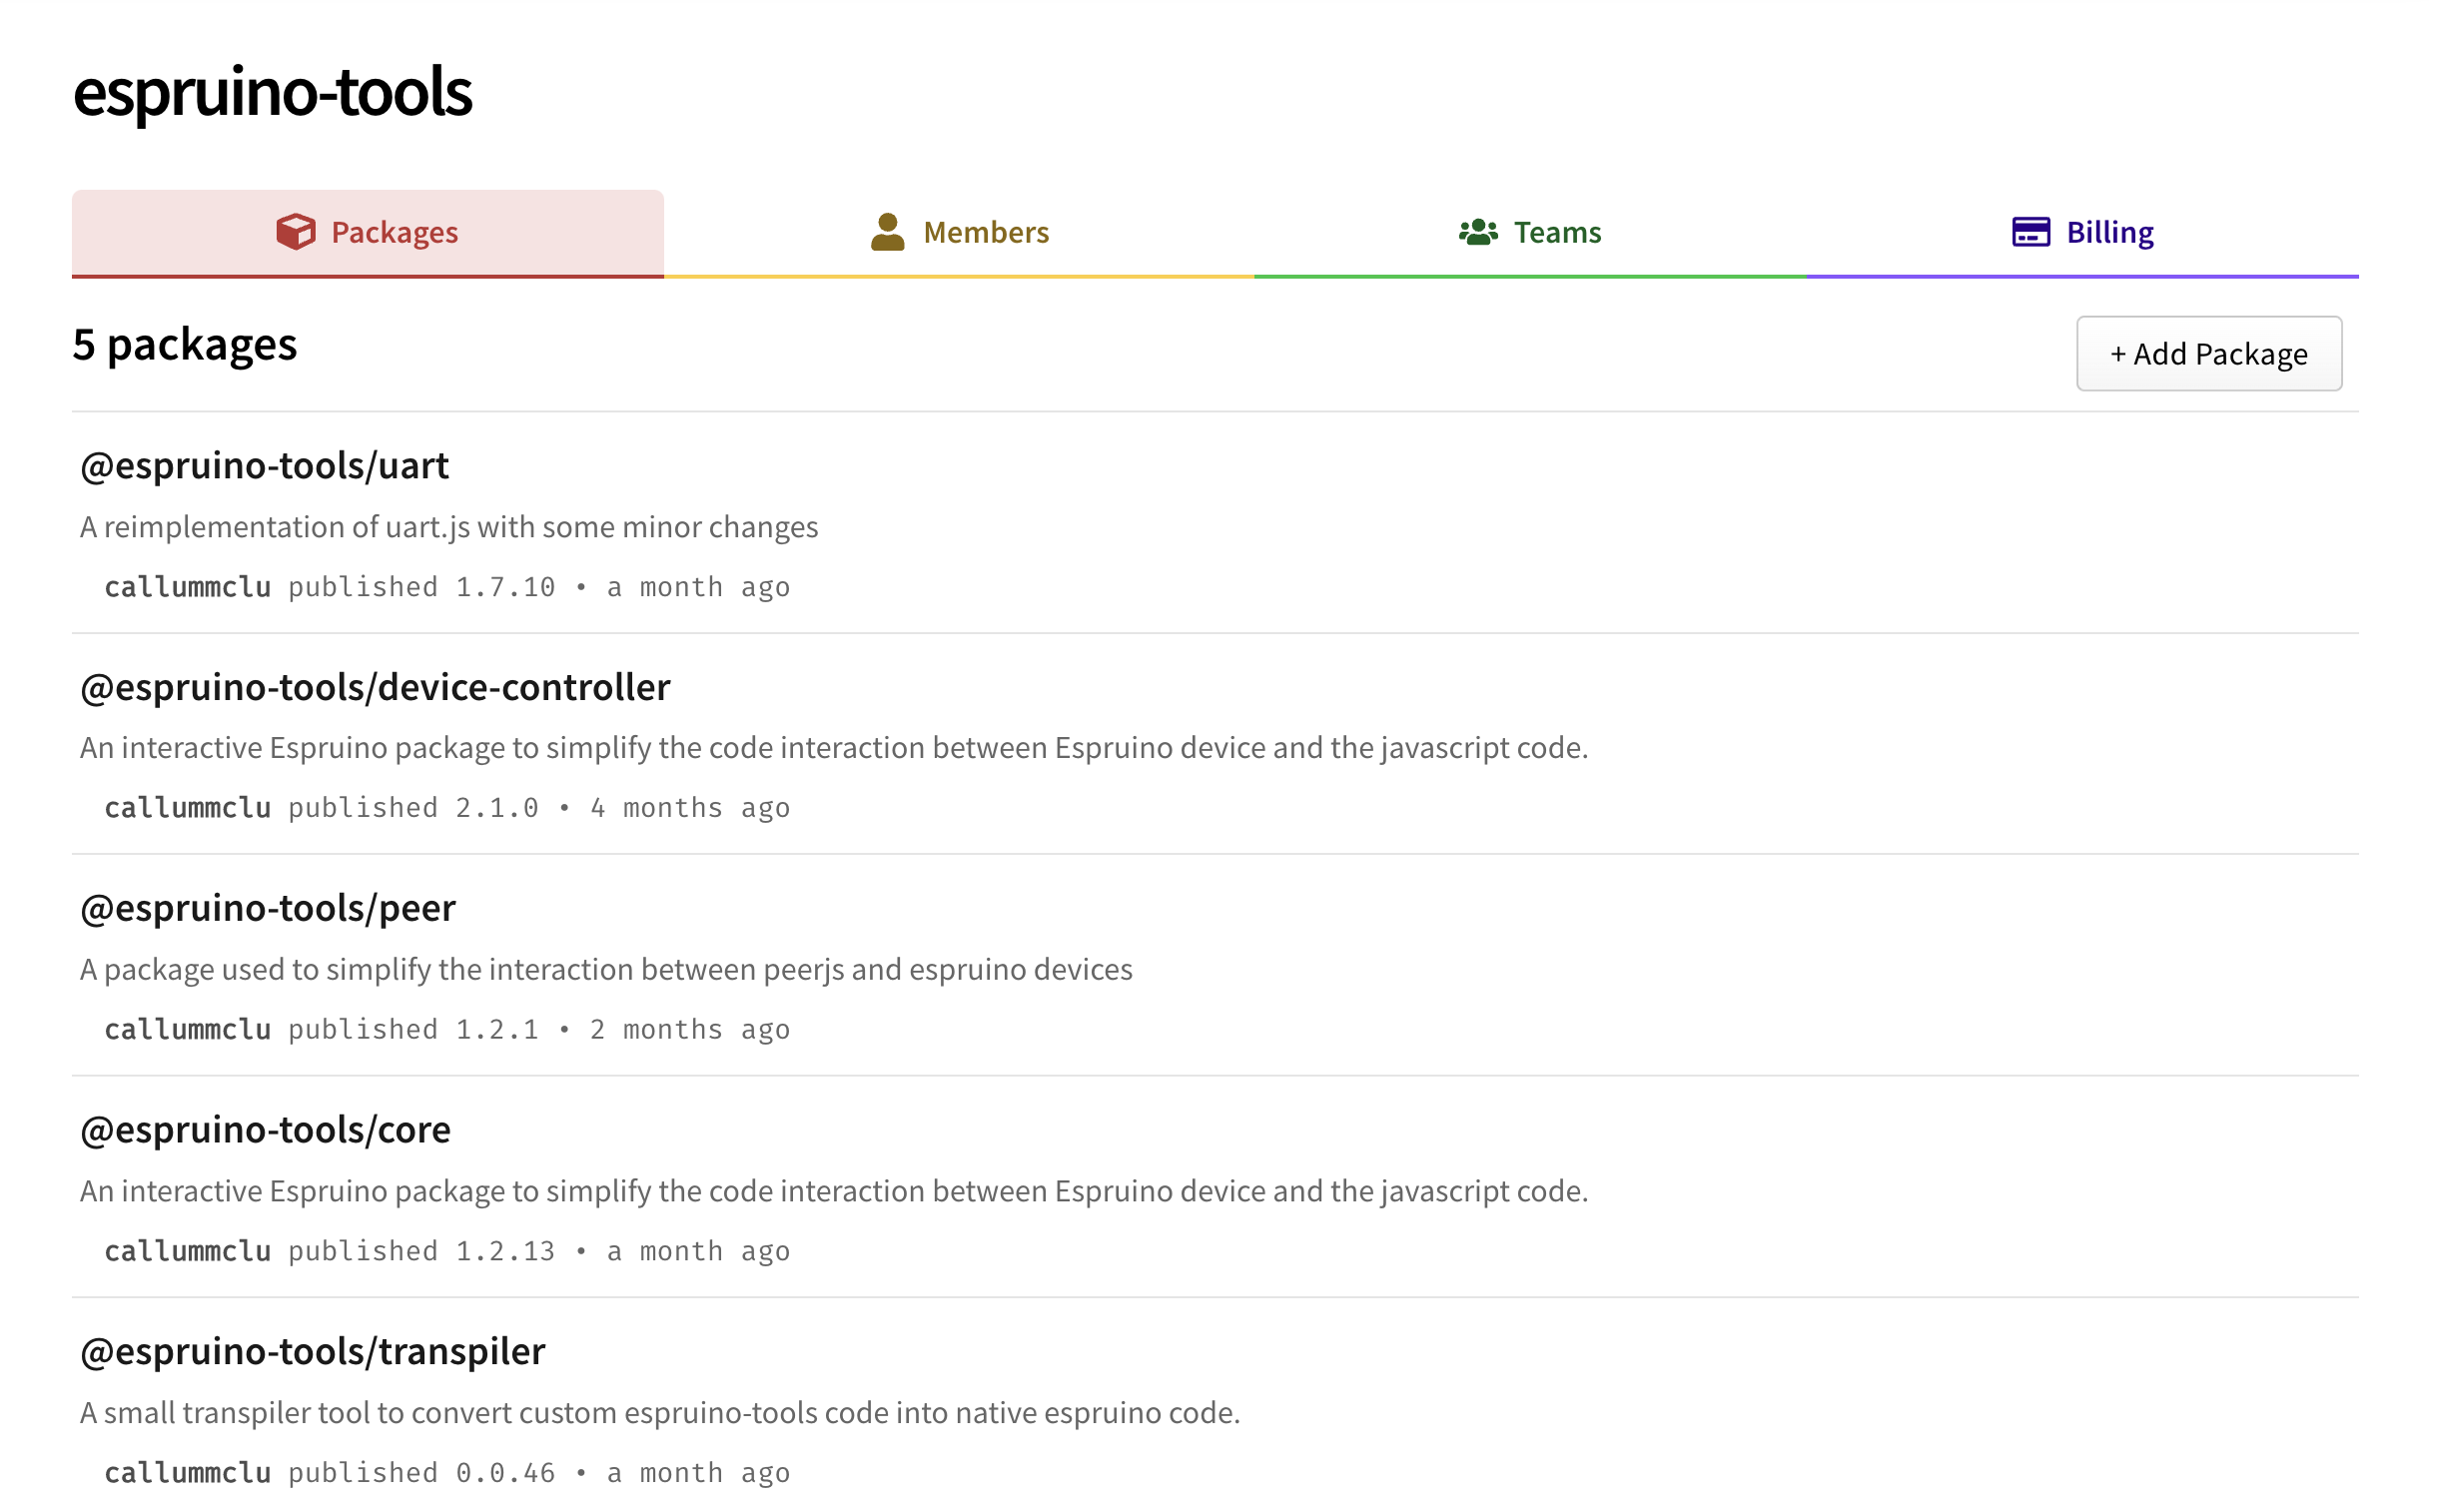
\includegraphics[width=10cm]{dissertation/images/npm-scoped-packages.png}
    \caption{NPM scoped package Organisation}
    \label{fig:npmorg}
\end{figure}

\section{Packaging Naming scheme}
A massive factor when developing NPM packages is how to correctly name them to both provide context for functionality without adding additional confusion. Whilst developing the package ecosystem 2 main questions arose, how can we group packages together and how do other successful package ecosystems do this? As previously stated in the sub-section 4.2.2 NPM's scoped packages allowed for a clean and clear representation of package grouping through the organisations' name, this solved this issue. Following this further research was done into successful package ecosystems such as \href{https://babeljs.io/}{babel}, \href{https://jestjs.io/}{jest} and \href{https://sentry.io/welcome/}{Sentry}. From this research, there seemed to be a clear unspoken naming convention for NPM packages this included.
\begin{itemize}
    \item \textbf{"core"} name for the main package.
    \item short descriptive package names, usually a single word when appropriate.
\end{itemize}

The criteria provided from this research provided clear instructions on how the packages within this ecosystem should be named.

\section{Package Versioning}
To ensure the package was versioned correctly resulting in a reliable and secure experience for the end users an approach was taken from the official \href{https://docs.npmjs.com/about-semantic-versioning
}{NPM website}. This approach is shown in figure \ref{fig:NPM-versioning}

\begin{figure}[!ht]
    
\begin{center}
\begin{tabular}{|p{2.25cm}|p{7.25cm}|p{3.25cm}|}
 \hline
 \textbf{Update Type} & \textbf{Example Change} & \textbf{Version Change} \\
 \hline
 \hline
Bug Fix & Package updates or security fixes  &  x.x.1  \\
 \hline
Minor change & Non breaking additions such as functionality extension  &  x.1.x  \\
 \hline
Major change & Breaking changes such as changes in syntax, anything that is not backwards compatible  &  1.x.x  \\
 \hline
\end{tabular}
\end{center} 
    \caption{NPM Package Versioning}
    \label{fig:NPM-versioning}
\end{figure}

\section{NPX Tool Repositories}
The NPX Tool aimed to generate directories based on a user's needs and aims to provide a wide variety of options to facilitate this. After exploring how React's \textbf{create-react-app} approached this problem we can see the team has opted to have directories for the \href{https://github.com/facebook/create-react-app/tree/main/packages/cra-template}{plain javascript implementation} and the \href{https://github.com/facebook/create-react-app/tree/main/packages/cra-template-typescript}{typescript implementation}. This dynamic approach provided by React's \textbf{create-react-app} inspired the design of the \textbf{create-espruino-app} in the following ways.

\subsection{Git sub-modules}
Whilst the \textbf{create-react-app} tool kept its templates within the same repository I believed this was a restrictive method and provided many downsides one of which being a bloated repository making it more difficult for developers to fully understand how the tool worked. To resolve this issue an approach using git sub-modules was taken. Git sub-modules allow for incorporating separate git repositories within one another; this would allow for the NPX tool repository to be linked to separate template repositories.

By using a single repository per template we are able to update file structure, patch security bugs, and package dependencies and even change the best methods of approaching building the web app without having to re-publish the tool. This approach also allowed for branching to be used for further flags on templates such as \textit{--clean-install} or \textit{--peer} meaning the end product would have a cleaner setup with more readable repositories.

\subsection{Flags}
Within CLI tool development CLI flags are used to provide user input and customise the output of a command. In the case of the tool developed CLI flags are proposed to provide the end developer with as much control over their new project as possible by incorporating different templates for popular web frameworks, easy access to a functioning setup of the peer package and even options for advanced allowing them to start off with a clean slate. These tags consist of:

\subsubsection{template}\hfill\\
The template tag allows developers to get started with a template built with one of 4 options: Plain Javascript, TypeScript, React or Vue. These options were chosen due to consideration from figure \ref{fig:js_framework_lib_comp} whilst maintaining the need for plain javascript/typescript templates to allow for flexibility when not working with a framework. The template tag allows for package-specific formatting to be set up by default this could be routing or general file structure.

\text \\

\subsubsection{peer}\hfill\\
The peer tag allows users to get started with the peer package without having to worry about the restrictions of the WebRTC API such as SSL requirements or separate pages needing to be hosted for it to function properly.

\text \\

\subsubsection{clean-install}\hfill\\
clean-install is a flag which is aimed at not restricting the usage of the tool to just beginners by allowing a directory to be populated just by the required packages removing any example splash pages presented by the standard package. The goal of this flag was to not alienate more advanced programmers whilst still giving them the benefits of the tool.

\section{UI/UX Improvements}
Previous implementations of device connection through packages such as \href{https://www.espruino.com/UART.js}{uart.js} all fall short when it comes to user experience presenting users with a badly designed modal with little to no control for leaving the modal without processing a request first. To tackle this problem with inspiration from the react component library \href{https://mantine.dev/}{Mantine} a Figma prototype was prepared to improve the user interface and experience of the mandatory modal. In figure \ref{fig:old-connection-modal} we can see the old design with layout issues and a general lack of responsive design. In figure \ref{fig:new-connection-modal} we can see the newly thought-out design prototype incorporating an option to close the modal with a clearer design. 

\begin{figure}[!ht]
\centering
\begin{minipage}{.5\textwidth}
  \centering
  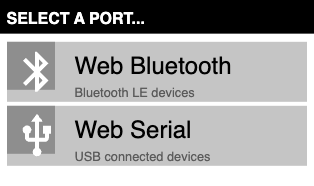
\includegraphics[width=6cm]{dissertation/images/old-modal-design.png}
  \captionof{figure}{Old Connection Modal}
  \label{fig:old-connection-modal}
\end{minipage}%
\begin{minipage}{.5\textwidth}
  \centering
  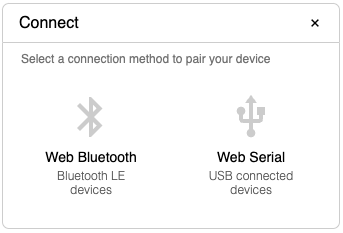
\includegraphics[width=6cm]{dissertation/images/new-modal-design.png}
  \captionof{figure}{New Connection Modal}
  \label{fig:new-connection-modal}
\end{minipage}
\end{figure}

This design process incorporated the previously mentioned feedback-driven approach going through many iterations to reach a final product with feedback from my supervisor who had previously mentioned issues with the prior connection modal.


%==================================================================================================================================
\chapter{Tools / Technologies}

This project was heavily dependent on the tools and technologies used within it as they acted as the fundamental building block which allowed it to be constructed.

\section{General}

The packages discussed below are used throughout the full ecosystem and help provide the vital structure of the package development.

\subsection{Typescript}
\href{https://www.typescriptlang.org/}{Typescript} \text offers several benefits over JavaScript when building a software package. It is a statically typed superset of JavaScript, providing improved code quality through static typing and a better understanding of large code bases through its type system. Typescript also offers better scalability with features like interfaces, classes, and modules, as well as better tooling support through better integration with modern development tools. Additionally, Typescript includes features that are part of upcoming versions of JavaScript, making code written in it future-proof.

\subsection{NPM}
\text Using the Node Package Management (\href{https://www.npmjs.com/}{NPM}) system when developing a JavaScript application presents numerous benefits. NPM eases the management of packages, guaranteeing the right version is installed correctly. The NPM network boasts a significant community of developers and a vast collection of programs, minimizing the need for repeated efforts and making it easy to integrate new features. NPM standardizes the system for versioning packages and enables the seamless distribution of programs to the community. The adoption of NPM also enables the automation of processes like building, testing, and deploying packages, reducing the workload associated with managing the project.


\subsection{UNPKG}
\text The utilization of inline JavaScript imports through \href{https://unpkg.com/}{UNPKG} provides numerous advantages. The ability to integrate small amounts of code through inline imports enables a fast and straightforward method for experimenting with various components and evaluating different solutions. Utilising both inline imports and NPM package imports simultaneously presents a versatile and efficient development process, empowering developers to select the most suitable approach for their project needs.

\subsection{Azure DevOps}
 \href{https://azure.microsoft.com/en-us/products/devops}{Azure DevOps} \text is a unified platform for software development that consolidates various tools and services. It offers a complete solution for source control, continuous integration/testing/deployment, and project management. Azure DevOps streamlines the development process by providing features such as automated builds, continuous deployment, and team collaboration, outperforming alternative approaches that utilize individual tools like Jenkins or Jira.

\subsection{Webpack}
\href{https://webpack.js.org/}{Webpack} \text is a popular module bundler used within node.js projects. It offers the ability to build JavaScript directories into efficiently bundled files by utilising methods like tree shaking, scope hoisting and file minification. A bonus of Webpack is the vast platform of packages allowing for incorporating other static files such as HTML and CSS into bundles, alongside this Webpack is heavily used in effectively building pre-processors and transpilers such as TypeScript and \href{https://sass-lang.com/}{SASS} which are both heavily used within the project. On top of this, Webpack's babel plugin allows for the usage of the latest version of ECMAScript whilst still compiling into ES5-compatible code. There are several Webpack alternatives such as \href{https://rollupjs.org/}{Rollup} and \href{https://parceljs.org/}{Parcel}; Webpack was chosen due to its large ecosystem of plugins, vast documentation and wider feature set. 

\subsection{React}

 \href{https://reactjs.org/}{React} \text is a popular and widely used JavaScript library utilised for building user interfaces. Developed by Facebook, react has gained widespread adoption within the professional software field due to its flexibility and robust core feature set. React was chosen due to its component-based architecture allowing for a shared and consistent design throughout the web applications built into the project as well as its wide variety of packages. React has many competitors such as \href{https://vuejs.org/}{Vue} and \href{https://angular.io/}{Angular} all of which achieve the same goal of creating complex user interfaces whilst boasting impressive core feature sets of their own but due to React's ease of learning and wide adoption, it made the most sense to pick for an open-source project. Below we can see a survey taken by \href{https://2022.stateofjs.com/en-US/libraries/front-end-frameworks/}{stateofjs} highlighting the usage of React over the past six years showing the popularity of it in comparison to Vue and Angular.

\begin{figure}[!ht]
    \centering
    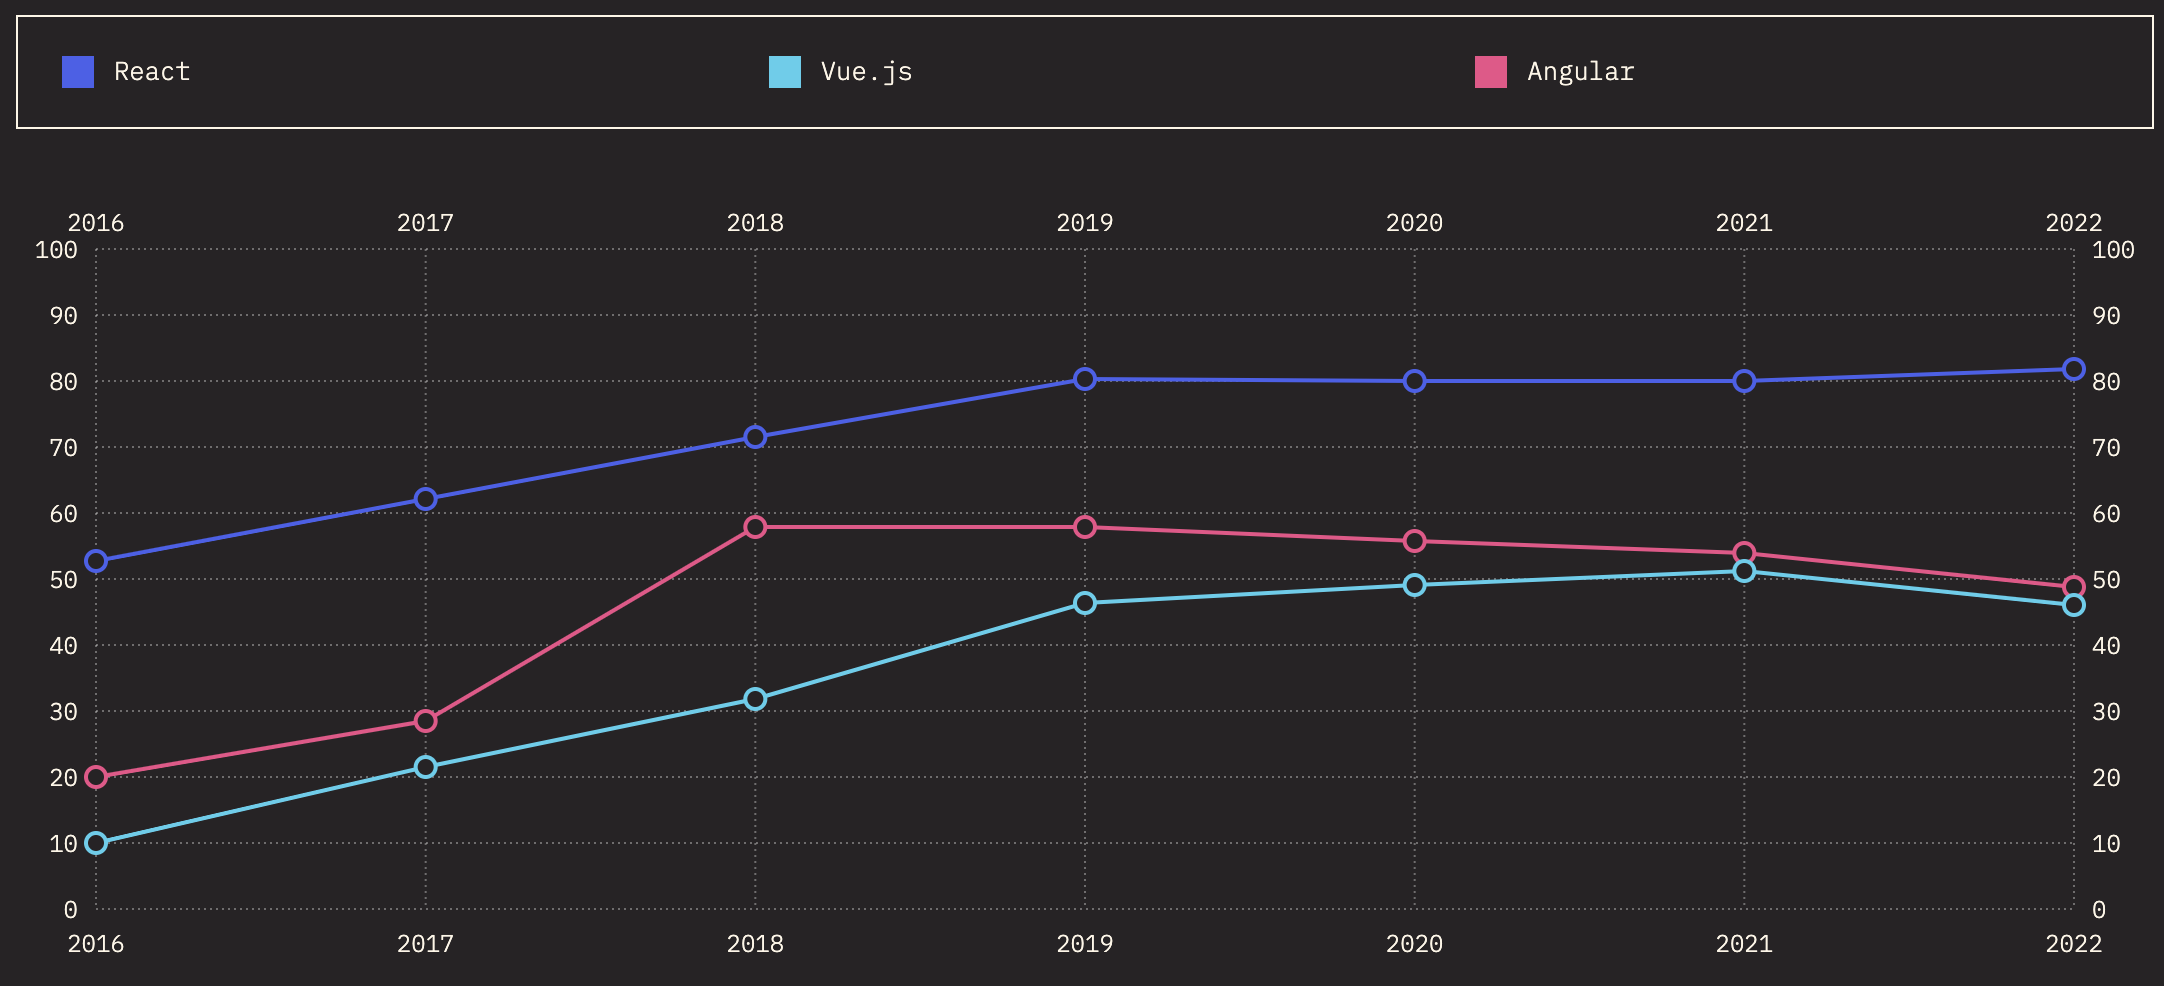
\includegraphics[width=13cm]{dissertation/images/framework_popularity_comparison.png}
    \caption{stateofjs JavaScript framework/library usage comparison}
    \label{fig:js_framework_lib_comp}
\end{figure}

\subsection{Husky}
\href{https://typicode.github.io/husky/#/}{Husky} is an open-source package which allows for easy control over git hooks within JavaScript projects. Husky allows for a developer to run commands on specific \href{https://git-scm.com/docs/githooks}{git hooks} such as \textit{pre-commit} and \textit{pre-commit-merge}. The addition of husky to a project allows for actions such as code testing and linting, presenting a solution to developers forgetting to perform these tasks before pushing code through the pipeline. Husky provides an ecosystem full of plugins and packages that can be used to improve the development of JavaScript packages.

\subsection{Standard Version}
\href{https://github.com/conventional-changelog/standard-version#readme}{Standard Version} is a package which allows for the automatic versioning of a project or packages alongside the automatic generation of a change-log based on commit messages. When used in tandem with Husky Standard Version provides a platform which eliminates the need for developers to manually perform package versioning or the difficult task of ensuring a change log is always up to date.

\section{CLI tool}

The CLI tool takes a different approach in development to the NPM packages as there is a requirement to be run through the command line.

\subsection{NPX }
\href{https://docs.npmjs.com/cli/v7/commands/npx}{NPX} is a command line package runner allowing for the execution of node-based JavaScript packages through a specified command. This has avid usage within the javascript development scene for building starting point directories, popular examples include React's \href{https://reactjs.org/docs/create-a-new-react-app.html}{create-react-app} and Vue's \href{https://cli.vuejs.org/}{vue-cli} to name a few.

\section{Peer}

Integrating a peer-to-peer connection without utilising a self-built and hosted back-end system presented a problem.

\subsection{peerJS}
\href{https://peerjs.com/}{PeerJS} provides an all-in-one solution which utilises WebRTC removing the issue of building a homemade WebSocket back-end system to allow for real-time communication between devices this approach allows developers to keep the simplicity of hosting static files without having to worry about the maintenance and cost of hosting of a back-end system.

\subsection{qrcode Package }
\text Building a bespoke QR code generator did not make sense for this project due to time constraints; to bypass this issue a pre-built solution \href{https://github.com/soldair/node-qrcode#readme}{qrcode} was used. qrcode provides a lightweight solution to building SVG QR codes easily embeddable into a web page. The package converts any given text into a scannable QR code including but not limited to urls and phone numbers. 

\section{Documentation }

\subsection{Docusaurus}
\href{https://docusaurus.io/}{Docusarus} is a documentation generator that takes inspiration from React to provide a platform for easily building and maintaining documentation websites. Developed by Facebook, it is a widely adopted solution for creating high-performing and highly customisable documentation sites thanks to its \href{https://mdxjs.com/}{MDX} support. MDX similar to \href{https://reactjs.org/docs/introducing-jsx.html}{JSX} used within React is a file format which allows the inclusion of componentised JSX within markdown allowing for consistent design with reduced development time. Additionally, Docusarus by default allows for \href{https://www.algolia.com/}{algolia} search integration, an option which adds a full site search to the static site to allow for site-wide searching functionality without the overhead of a backend system to support it. When comparing Docusaurus to the competition, other documentation generators such as \href{https://jekyllrb.com/}{jekyll} and \href{https://www.sphinx-doc.org/en/master/}{sphinx} Docusaurus despite being the newest competitor of the bunch has a wide community and dramatically increases the customizability and performance when compared to the others resulting in documentation sites that arent which can be better custom fit to the projects overall branding and style.


\section{Transpiler}

Building a transpiler is a difficult task to do well, fortunately, there are many packages which can help with steps throughout the processes of parsing, tokenising and code generation allowing for more focus to be put on what needs to be changed.

\subsection{Esprima }
\href{https://esprima.org/}{Esprima} is a JavaScript parser written in JavaScript with the aim of simplifying parsing given ECMAScript 2016 code. Esprima provides functionality for the developer to tokenise and parse JavaScript code into an Abstract Syntax Tree (AST) to the Mozilla (\href{https://developer.mozilla.org/en-US/}{MDN}) JavaScript specification. By providing a comprehensive documentation site Esprima is able to take the hassle out of creating a parser for JavaScript allowing developers to not have to reinvent the wheel and instead put focus on altering the syntax trees to implement their syntax extensions/alterations. 

\subsection{EsCodeGen }
\href{https://github.com/estools/escodegen#readme}{EsCodeGen} is a code generator built for JavaScript which has the sole purpose of converting Mozilla (MDN) compatible Abstract Syntax Trees (ASTs) into readable JavaScript code. EsCodeGen has support for ECMAScript 2016 making it directly compatible with Esprima. This package was utilised due to Esprima's lack of a code generator and avoids the requirement of building a crude module to generate code from the generated ASTs.

%==================================================================================================================================
\chapter{Implementation}

\text Through the analysis of the project's specification a decision was made to separate functionality that is unrelated or can be used independently into their own packages or web applications. This approach resulted in the development of the following packages and web applications shown in figures \ref{fig:packages} and \ref{fig:webapps}.

\begin{figure}[!ht]
    
\begin{center}
\begin{tabular}{|p{2.25cm}|p{5.25cm}|p{5.25cm}|}
 \hline
 \multicolumn{3}{|c|}{Packages} \\
 \hline
 Name  & GitHub repository& Documentation\\
 \hline
Core & \href{https://github.com/espruino-tools/core}{espruino-tools/core}  & \href{https://documentation-xi-liard.vercel.app/docs/category/core}{docs/category/core}  \\

UART & \href{https://github.com/espruino-tools/uart}{espruino-tools/uart}  & \href{https://documentation-xi-liard.vercel.app/docs/category/uart}{docs/category/uart}  \\

Peer & \href{https://github.com/espruino-tools/peer}{espruino-tools/peer}  & \href{https://documentation-xi-liard.vercel.app/docs/category/peer}{docs/category/peer}  \\

Transpiler & \href{https://github.com/espruino-tools/transpiler}{espruino-tools/transpiler}  & \href{https://documentation-xi-liard.vercel.app/docs/category/transpiler}{docs/category/transpiler}  \\

CLI Tool &  \href{https://github.com/espruino-tools/create-espruino-app}{espruino-tools/create-espruino-app}  & \href{https://documentation-xi-liard.vercel.app/docs/category/create-espruino-app}{docs/category/create-espruino-app}  \\
 \hline
\end{tabular}
\end{center} 
    \caption{Packages}
    \label{fig:packages}
\end{figure}

\begin{figure}[!ht]
\begin{center}
\begin{tabular}{|p{2.25cm}|p{5.25cm}|p{5.25cm}|}
\hline
\multicolumn{3}{|c|}{Web Apps} \\
 \hline
 Name & GitHub repository & Site Link\\
 \hline
Online IDE & \href{https://github.com/espruino-tools/online-environment}{espruino-tools/online-environment} & \href{https://online-environment.vercel.app/}{online-environment.vercel.app} \\
Demo's Hub & \href{https://github.com/espruino-tools/demos}{espruino-tools/demos}  & \href{https://demos-mu.vercel.app/}{demos-mu.vercel.app} \\
Documentation & \href{https://github.com/espruino-tools/documentation}{espruino-tools/documentation} & \href{https://documentation-xi-liard.vercel.app/}{documentation-xi-liard.vercel.app} \\
 \hline
\end{tabular}
\end{center}
\caption{Web Apps}
\label{fig:webapps}
\end{figure}

Each of the packages has a unique dependency on each other, this choice of structure allows users to get involved at any step and even develop their own solutions to improve their own custom workflow, the dependency graph is shown in figure \ref{fig:package_dep_graph}

%========================
%=
%= 
%= IMAGE LUCID SPARK FOR REWORK
%= https://lucid.app/lucidchart/3338b1b0-2b62-481b-abb9-bbf9ce7b7a7d/edit?rtempr=1&invitationId=inv_25f074ac-b765-41ec-999b-6795aa3640dc&page=0_0#
%= 
%= 
%========================

\begin{figure}[!ht]
    \centering
    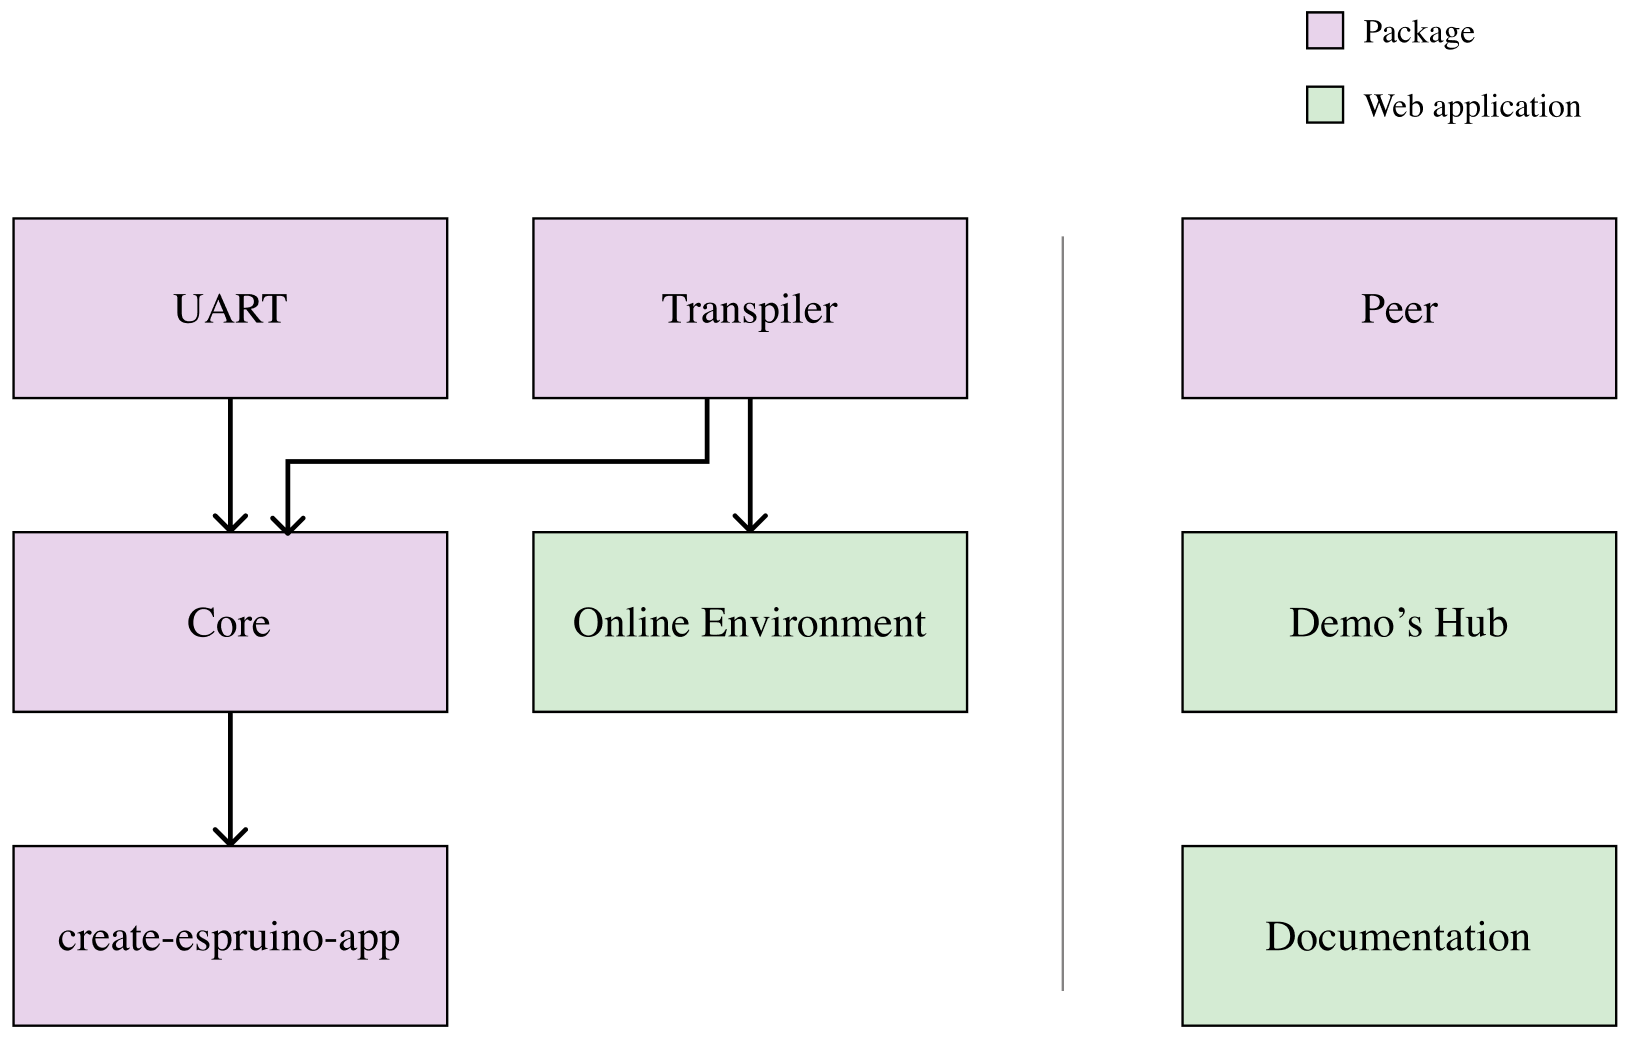
\includegraphics[width=10cm]{dissertation/images/Package_dependency_graph.jpeg}
    \caption{Dependency Graph}
    \label{fig:package_dep_graph}
\end{figure}

The packages and web applications above serve as a general view of the structure of the ecosystem the following will showcase the functionality of the packages/web applications in more detail.

\section{Packages}
A small introduction of the packages and why this approach was taken:

\begin{itemize}
    \item package approach, splitting functionality into independent parts, UNIX ideology reference.
\end{itemize}

\subsection{core}

\text What does it do.
\begin{itemize}
    \item removes need to directly send strings of code to a device.
    \item removes need for waits and provides an asynchronous model for data transfer
    \item provides a simplified approach to developing with espruino devices, \textbf{EXPLAIN WHY}.
\end{itemize}
\\
\textbf{What is impressive about it.} 
\begin{itemize}
    \item removes any confusion by incorporating everything you need into a single import based on device.
    \item allows for easy development of new devices via inheritance incorporating all basic functionality of the device (lightweight as well).
\end{itemize}
\subsection{peer}

\textbf{What does it do.}
\begin{itemize}
    \item WebRTC
    \item simplify the interaction between mobile devices and web browsers (QR Code).
\end{itemize}
\\
\textbf{What is impressive about it.}
\begin{itemize}
    \item easy to add to a site, simple configuration.
\end{itemize}
\subsection{uart}

\textbf{What does it do.}
\begin{itemize}
    \item Connection between Espruino devices and the webbrowsers
    \item improved user interaction with the package, (UI/UX)
    \item Overhaul of old package using modern javascript
\end{itemize}
\\
\textbf{What is impressive about it.}
\begin{itemize}
    \item utilises modern ECMAScript classes, allowing users to take advantage of inheritance for building their own UART implementations removing any issues with 
\end{itemize}

\subsection{create-espruino-app}

\textbf{What does it do.}
\begin{itemize}
    \item provides a simple one line command for users to get started. 
    \item provides a series of flags to customise the users development style from clean installing where no boilerplate files are provided to starting up a peer package directory.
\end{itemize}
\\
\textbf{What is impressive about it.}
\begin{itemize}
    \item Covers multiple modern development frameworks such as react and vue
\end{itemize}
\subsection{Transpiler}

\textbf{What does it do.}
\begin{itemize}
    \item Provides platform for writing core code and converting into native espruino code.
\end{itemize}
\\
\textbf{What is impressive about it.}
\begin{itemize}
    \item works as importable package and runnable CLI, allowing for full directory conversion similar to other transpiler/preprocessors such as typescript or the older coffeescript.
\end{itemize}

\section{Web Apps}

\text small paragraph about why web apps are required in this project, mention:

\begin{itemize}
    \item describe what packages do
    \item show users what the packages can do and how they can do it themselves
    \item provide an environment for users to test out functionality without committing to a project.
\end{itemize}

\subsection{online IDE}

\textbf{What does it do.}
\begin{itemize}
    \item Provides environment for online development similar to online compiler X.
\end{itemize}
\\
\textbf{What is impressive about it.}
\begin{itemize}
    \item showcases code saved on device
    \item showcases transpiled code, can be used for better understanding of the "lower level" code.
\end{itemize}

\subsection{Demo's Hub}
\textbf{What does it do.}
\begin{itemize}
    \item provides a hub for new or experienced users to browse projects built with espruino tools with easy downloading and a code viewer to see the process
\end{itemize}
\\
\textbf{What is impressive about it.}
\begin{itemize}
    \item PR based adding to site, no need for a back-end Static site generation.
    \item something about configuration file for page population.
\end{itemize}

\section{Documentation}
\textbf{What does it do.}
\begin{itemize}
    \item place for all documentation all in one well organised place.
    \item full site searching
\end{itemize}
\\
\textbf{What is impressive about it.}
\begin{itemize}
    \item everything is built with components allowing for new pages to be built with next to no need for configuration or hassle.
\end{itemize}
\section{CI/CD}
\text The CI/CD pipeline built provides a platform that streamlines the development process of the packages, this process provides the structure for how the packages are tested and prepared before deployment alongside how they are deployed leaving the developer to focus on the programming and less on the semantics of deploying an application. This is shown below in Figure \ref{fig:CICDPipeline}

\begin{figure}[!ht]
    \begin{center}
        
    
    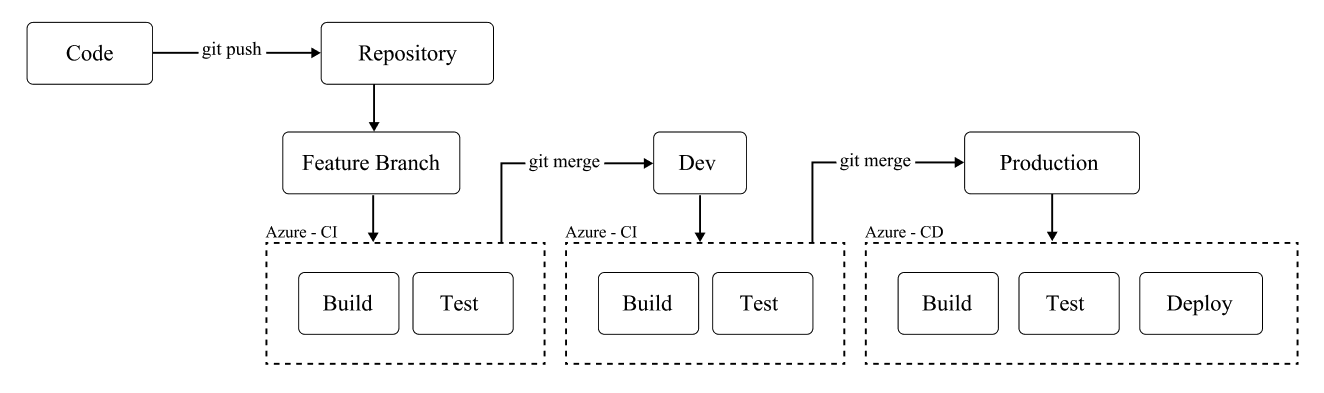
\includegraphics[width=14cm]{dissertation/images/CICD-structure.png}
    \end{center}
    \caption{CI/CD Pipeline}
    \label{fig:CICDPipeline}
\end{figure}
\\
\textbf{What does it do.}
\begin{itemize}
    \item automated testing, building, deployment.
\end{itemize}
\\
\textbf{What is impressive about it.}
\begin{itemize}
    \item automated deployment.
\end{itemize}


\section{Testing}
\text JEST, javascript testing suite. Cypress,Front end testing suite, Mocking, JSDOM. (this may only be applicable for demo site and online IDE.
\\
\textbf{What does it do.}

\\
\textbf{What is impressive about it.}



\section{Deployment}
\subsection{Packages}
\text How the packages are deployed using azure pipelines ,npm and unpkg to host package. using webpack for building minified and non minified packages (from typescript).

\begin{figure}[!ht]
    \begin{center}
    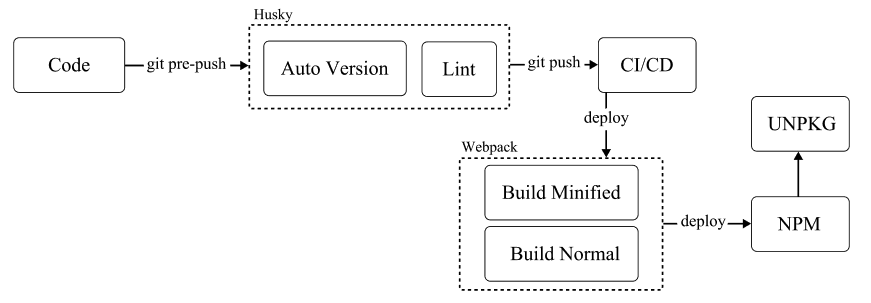
\includegraphics[width=14cm]{dissertation/images/Deployment.png}
    \end{center}
    \caption{Deployment}
    \label{fig:deployment}
\end{figure}
\\
\textbf{What does it do.}
\begin{itemize}
    \item deployed via CI/CD through NPM publish, minified script is hosted automatically through UNPKG
\end{itemize}
\\
\textbf{What is impressive about it.}
\begin{itemize}
    \item automated versioning through husky.
    \item automated change-log based on commit messages.
    \item automated deployment via secondary pipeline for every package which runs on production merge after original pipeline run on development, helped via branch protection.
\end{itemize}
\subsection{Web Apps}
\text How the web apps are deployed. Vercel, what is Vercel and why use it?
\\
\textbf{What does it do/what is impressive}
\begin{itemize}
    \item runs its own CI/CD on top of mine
    \item provides deployments for development versions to test features before full production deployment.
\end{itemize}

\chapter{Evaluation} 
How good is your solution? How well did you solve the general problem, and what evidence do you have to support that?

\section{User Feedback}
\subsection{Core}
\begin{itemize}
    \item Code upload
\end{itemize}
\subsection{Peer}
\subsection{UART}
\begin{itemize}
    \item issues with transfer delays
\end{itemize}
\subsection{NPX Tool}
\begin{itemize}
    \item deployment
    \item tag usage (peer not working, https issue)
    \item bundling of static assets (images)
\end{itemize}
\section{Core}
\subsection{Speed Comparison}
How much slower is using this package instead of writing natively, use online IDE vs espruino IDE write the same code using both, measure lines of code taken, code cleanness if possible and time taken to run.
\section{Peer}
\subsection{Speed Comparison}
How much does sending requests over peer connection affect performance, how does this compare to more conventional Bluetooth controller devices 
\subsection{Code changes from peerjs}
\begin{itemize}
    \item Cleaner syntax comparison, development time
    \item 
\end{itemize}
\section{Transpiler}
Why was this approach better than the miniParser (get stats or measurements for both).
\begin{itemize}
    \item coverage (miniParser did not work on nested code with additional scopes)
    \item speed
\end{itemize}

%==================================================================================================================================
\chapter{Conclusion}    
Summarise the whole project for a lazy reader who didn't read the rest (e.g. a prize-awarding committee).
\section{Summary}
\section{Reflection}
\section{Future Work}
\subsection{Espruino device package}
\begin{itemize}
    \item run espruino tools code directly on device.
    \item usage of wide variety of non espruino tools ecosystem.
\end{itemize}
\subsection{Transpiler CLI}
\begin{itemize}
    \item Tool to convert whole project of espruino tools code to native espruino code.
\end{itemize}
\section{Limitation}

%==================================================================================================================================
%
% 
%==================================================================================================================================
%  APPENDICES  

\begin{appendices}
\chapter{Individual MOSCOW Analysis}


\label{appendix:MOSCOWAnalysis}

Below are the individual MOSCOW analysis of each project. These will go further into depth about the state of each individual project analysis and provide more detail surrounding the priorities.

%== CORE

\section{Core}
\subsection{Must Have}
\begin{itemize}
    \item Implement all device specific functionality into Device Objects
    \item Provide a more readable syntax for beginner users without restricting functionality
    \item Support TypeScript
    \item Be open-source
    \item Support any package import method (i.e. NPM, script tag imports)
\end{itemize}
\subsection{Should Have}
\begin{itemize}
    \item The ability to call on device functions that are already on the device.
    \item Functionality to gather device code in a readable manor, (gather functions on the device with parameters)
    \item upload code to the device.
\end{itemize}
\subsection{Could Have}
\begin{itemize}
    \item In-line documentation for package usage in IDE
\end{itemize}

%== UART

\section{UART}
\subsection{Must Have}
\begin{itemize}
    \item Improved UI/UX (cleaner modal, option to close modal)
    \item Support Typescript
    \item Be open-source
    \item Support any package import method (i.e. NPM, script tag imports)
\end{itemize}
\subsection{Should Have}
\begin{itemize}
    \item Speed Improvements (remove unused code, reduce package size, replace waits with promises)
    \item Improve device detection, current IOS detection does not work and WebBluetooth is not compatible with IOS.
    \item Use more readable javascript/typescript (original used bad code practices such as repeated code, bad variable names, global variables for everything)
\end{itemize}
\subsection{Could Have}
\begin{itemize}
    \item Call log to see what was last called on device.
    \item In-line documentation for package usage in local IDE.
\end{itemize}
\subsection{Would be nice to Have}
\begin{itemize}
    \item Options on creation for user specified maximum wiat time for device response.
\end{itemize}

%== PEER

\section{Peer}
\subsection{Must Have}
\begin{itemize}
    \item Support for both iOS and android smart devices.
    \item Support Typescript.
    \item Be open source.
    \item Support any package import method (i.e. NPM, script tag).
    \item Simplify setup of peerjs package to suit a standard use case without limiting the usage.

\end{itemize}
\subsection{Should Have}
\begin{itemize}
    \item Provide QR code for device connection.
    \item Support simultaneous front and back camera streaming.

\end{itemize}
\subsection{Could Have}
\begin{itemize}
    \item Provide notifications to show users connection has been initialised or closed.
    \item In-line documentation for package usage in IDE

\end{itemize}
\subsection{Would be nice to Have}
\begin{itemize}
    \item Have consistent styling with UART package.
\end{itemize}

%== TRANSPILER

\section{Transpiler}
\subsection{Must Have}
\begin{itemize}
    \item Support Typescript
    \item Be open source
    \item Support any package import method (i.e. NPM, script tag)
    \item Support standard language functionality such as variable declaration and code conversion of code within nested scopes.

\end{itemize}
\subsection{Should Have}
\begin{itemize}
    \item Convert code regardless of syntax errors (for usage with newly released commands in espruino spec that arent currently supported).
    \item Support modern javascript syntax such as classes and arrow functions.
    \item Have options to transpile modules or scripts.

\end{itemize}
\subsection{Could Have}
\begin{itemize}
    \item A CLI tool to build full directories into espruino native code.
    \item In-line documentation for package usage in IDE

\end{itemize}

%== CLI TOOL

\section{CLI Tool}
\subsection{Must Have}
\begin{itemize}
    \item utilise NPX to remove need for downloading and running applications, keeps it within the ecosystem of NPM.
    \item Be open source
    \item Create a working directory with the latest versions of the core package.

\end{itemize}
\subsection{Should Have}
\begin{itemize}
    \item Support multiple frameworks / coding templates such as typescript, react, vue and plain javascript.
    \item Have a template for peer setup allowing users to get started with the peer package.
    \item Error handling for incorrect command input to prevent a directory from being built on failure.

\end{itemize}
\subsection{Could Have}
\begin{itemize}
    \item Have clear progress letting the user know where the tool is in its installing progress.
\end{itemize}
\subsection{Would be nice to Have}
\begin{itemize}
    \item Support for custom templates via a github clone and set of commands to be run
\end{itemize}

%== ONLINE ENVIRONMENT

\section{Online Environment}
\subsection{Must Have}
\begin{itemize}
    \item Be open source
    \item Support live development being able to run code directly on device.
    \item Show terminal output

\end{itemize}
\subsection{Should Have}
\begin{itemize}
    \item Ability to see transpiled code.
    \item upload code from computer.
    \item save code to computer.
    \item Ability to see code on the device.

\end{itemize}
\subsection{Could Have}
\begin{itemize}
    \item Ability to save code editor code to device.
\end{itemize}
\subsection{Would be nice to Have}
\begin{itemize}
    \item A progressive web app conversion to allow for the site to be used as a local app for offline development.
\end{itemize}

%== DEMOS HUB

\section{Demos Hub}
\subsection{Must Have}
\begin{itemize}
    \item Be open source
    \item Support community uploads of demos.
    \item Show video of demo
    \item Show code from specified repository in read-only code editor.

\end{itemize}
\subsection{Should Have}
\begin{itemize}
    \item Have optionally specified links.
\end{itemize}
\subsection{Could Have}
\begin{itemize}
    \item config file to specify all information required to build the page.
\end{itemize}
\subsection{Would be nice to Have}
\begin{itemize}
    \item A page for showing users how to upload their own demos.
\end{itemize}

%== DOCUMENTATION

\section{Documentation}
\subsection{Must Have}
\begin{itemize}
    \item Be open source (Allow community edits)
    \item Accurately describe functionality of all packages
\end{itemize}
\subsection{Should Have}
\begin{itemize}
    \item Have searching functionality
    \item Provide examples of code working
\end{itemize}

\chapter{Project demos}


\label{appendix:projdemos}

\section{Core}

\begin{figure}[!ht]
    \centering
    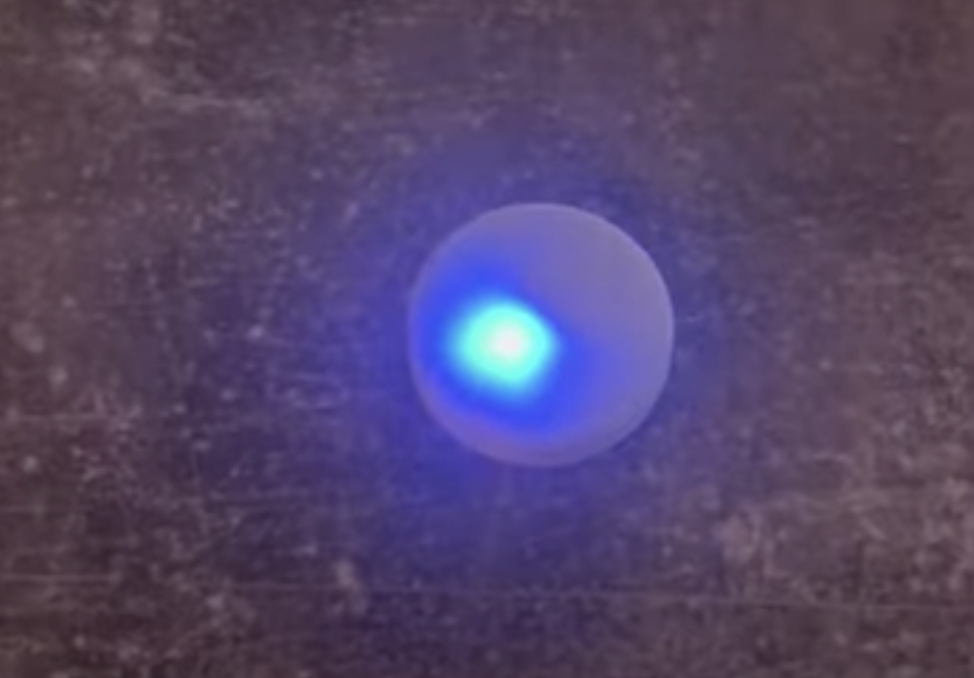
\includegraphics[width=8cm]{dissertation/images/light-sensor-demo.png}
    \caption{\href{https://demos-mu.vercel.app/demo/light-sensor}{Light Sensor Demo}}
\end{figure}



\section{Peer}
\section{Transpiler}
\section{create-espruino-app}


\chapter{User Study Data}

\label{appendix:userstudydata}

\chapter{Student University Study}

\label{appendix:studentunistudy}
\end{appendices}

%==================================================================================================================================
%   BIBLIOGRAPHY   

% The bibliography style is abbrvnat
% The bibliography always appears last, after the appendices.

\bibliographystyle{abbrvnat}

\bibliography{l4proj}

\end{document}
